% !TeX program = pdflatex
% !BIB program = biber

\documentclass[
  a4paper,
  11pt,
  ngerman,
  parskip=half,
  bibliography=totoc,
  listof=totoc
]{scrreprt}

% ============================================================================
% PACKAGES
% ============================================================================

\usepackage[left=3cm,right=2.5cm,top=2.5cm,bottom=2.5cm]{geometry}
\usepackage[ngerman]{babel}
\usepackage{csquotes}
\usepackage{listings}
\usepackage{xcolor}
\usepackage{acronym}
\usepackage{amsmath, amssymb}
\usepackage{graphicx}
\graphicspath{{img/}}
\usepackage{booktabs}
\usepackage{hyperref}
\usepackage{float}

% Bibliografie mit IEEE-Stil
\usepackage[
  backend=biber,
  style=ieee,
  citestyle=ieee,
  natbib=true
]{biblatex}

\addbibresource{../DemoVideo_and_Documentation/Documentation.bib}

% ============================================================================
% CODE LISTINGS KONFIGURATION
% ============================================================================

\definecolor{codegreen}{rgb}{0,0.6,0}
\definecolor{codegray}{rgb}{0.5,0.5,0.5}
\definecolor{codepurple}{rgb}{0.58,0,0.82}
\definecolor{backcolour}{rgb}{0.95,0.95,0.92}

\lstdefinestyle{csharpstyle}{
    language=[Sharp]C,
    backgroundcolor=\color{backcolour},
    commentstyle=\color{codegreen},
    keywordstyle=\color{blue},
    numberstyle=\tiny\color{codegray},
    stringstyle=\color{codepurple},
    basicstyle=\ttfamily\small,
    breakatwhitespace=false,
    breaklines=true,
    captionpos=b,
    keepspaces=true,
    numbers=left,
    numbersep=5pt,
    showspaces=false,
    showstringspaces=false,
    showtabs=false,
    tabsize=4,
    frame=single,
    frameround=tttt
}
\lstset{style=csharpstyle}

% ============================================================================
% HYPERREF KONFIGURATION
% ============================================================================

\hypersetup{
    colorlinks=true,
    linkcolor=black,
    citecolor=black,
    filecolor=blue,
    urlcolor=blue,
    bookmarksnumbered=true
}

% ============================================================================
% TITLE PAGE INFORMATION
% ============================================================================

\title{Fragments of Silvaris: Ein 2D-RPG}
\subtitle{Dokumentation --- Spieleprogrammierung Projekt}
\author{Aaron Seitz (3006614) \and Robin Fitzek (3006199) \and Burak Yigit (3005865) \and Paul Weber (88487)}
\date{Februar 2026}

% ============================================================================
% DOCUMENT START
% ============================================================================

\begin{document}

% ============================================================================
% TITELSEITE
% ============================================================================

\newgeometry{left=2.5cm,right=2.5cm,top=2.5cm,bottom=2.5cm}

\begin{titlepage}
    \centering

    % HTW Logo
    
\includegraphics[width=0.3\textwidth]{htw.eps}\\[1cm]

    \vspace*{\fill}

    \textbf{\Large Hochschule Aalen}\\
    \textbf{\Large Technik und Wirtschaft}\\[2cm]

    \textbf{\huge Fragments of Silvaris}\\[0.5cm]
    \Large Ein 2D-RPG\\[2cm]

    \textbf{\large Dokumentation}\\
    Spieleprogrammierung --- Wintersemester 2025/2026

    \vspace{3cm}

    \large vorgelegt von

    Aaron Seitz (3006614)

    Robin Fitzek (3006199)

    Burak Yigit (3005865)

    Paul Weber (88487)

    \vspace{3cm}

    \large Februar 2026\\

    \vspace*{\fill}
\end{titlepage}

\restoregeometry

% ============================================================================
% ZUSAMMENFASSUNG (ABSTRACT)
% ============================================================================

\chapter*{Zusammenfassung}

Fragments of Silvaris ist ein 2D Action-RPG, das in Unity 6 entwickelt wurde und sich am Spieldesign des beliebten MMORPGs NosTale orientiert. Das Projekt zeigt die Umsetzung verschiedener Game Development Konzepte, mit besonderem Fokus auf intelligentes Gegner-Verhalten und durchdachte Spielmechaniken.

Das Herzstück des Spiels ist ein raycasting-basiertes System, das Gegnern ermöglicht, selbstständig um Hindernisse zu navigieren. Statt in Wänden stecken zu bleiben, können die Gegner dank multi-direktionaler Raycasts und dynamischer Ausweichlogik intelligent auf Hindernisse reagieren.

Weitere Highlights sind ein arc-basiertes Kampfsystem mit 60°-Angriffskegel, ein umfassendes RPG-System mit Inventar, Ausrüstung und Levelprogressionen, sowie ein dynamisches Audio-System, das zwischen Kampf- und Friedensmusik wechselt. Das Spiel bietet 10 miteinander verbundene Szenen mit Boss-Begegnungen, ein Journal-System für die Story und eine polierte Benutzeroberfläche.

Das Projekt wurde von einem Team über einen Zeitraum von Oktober 2025 bis Februar 2026 entwickelt und erfolgreich umgesetzt.

\newpage

% ============================================================================
% INHALTSVERZEICHNIS
% ============================================================================

\tableofcontents

% ============================================================================
% ABBILDUNGSVERZEICHNIS
% ============================================================================

\listoffigures

% ============================================================================
% TABELLENVERZEICHNIS
% ============================================================================

\listoftables

% ============================================================================
% ABKÜRZUNGSVERZEICHNIS
% ============================================================================

\chapter*{Abkürzungsverzeichnis}

\begin{acronym}
\acro{RPG}{Role-Playing Game}
\acro{NPC}{Non-Player Character}
\acro{UI}{User Interface}
\acro{URP}{Universal Render Pipeline}
\acro{XP}{Experience Points}
\acro{HP}{Health Points}
\acro{FPS}{Frames Per Second}
\acro{FSM}{Finite State Machine}
\acro{SFX}{Sound Effects}
\acro{MVP}{Minimum Viable Product}
\acro{A*}{A* Pathfinding-Algorithmus}
\acro{MVC}{Model-View-Controller}
\end{acronym}

\newpage

% ============================================================================
% HAUPTTEIL - SEITENZAHLEN VON ARABISCH
% ============================================================================

\pagenumbering{arabic}
\setcounter{page}{1}

% ============================================================================
% KAPITEL 1: ÜBERBLICK
% ============================================================================

\chapter{Überblick}

\section{Spielkonzept}

Fragments of Silvaris ist ein 2D Action-RPG mit Top-Down-Perspektive, entwickelt als Abschlussprojekt für die Vorlesung Spieleprogrammierung an der Hochschule Aalen. Das Spiel orientiert sich thematisch und mechanisch am beliebten MMORPG NosTale \cite{spieleprogrammierung_course}, kombiniert aber klassische 2D-RPG-Mechaniken mit modernen Game Development Standards.

\begin{figure}[H]
    \centering
    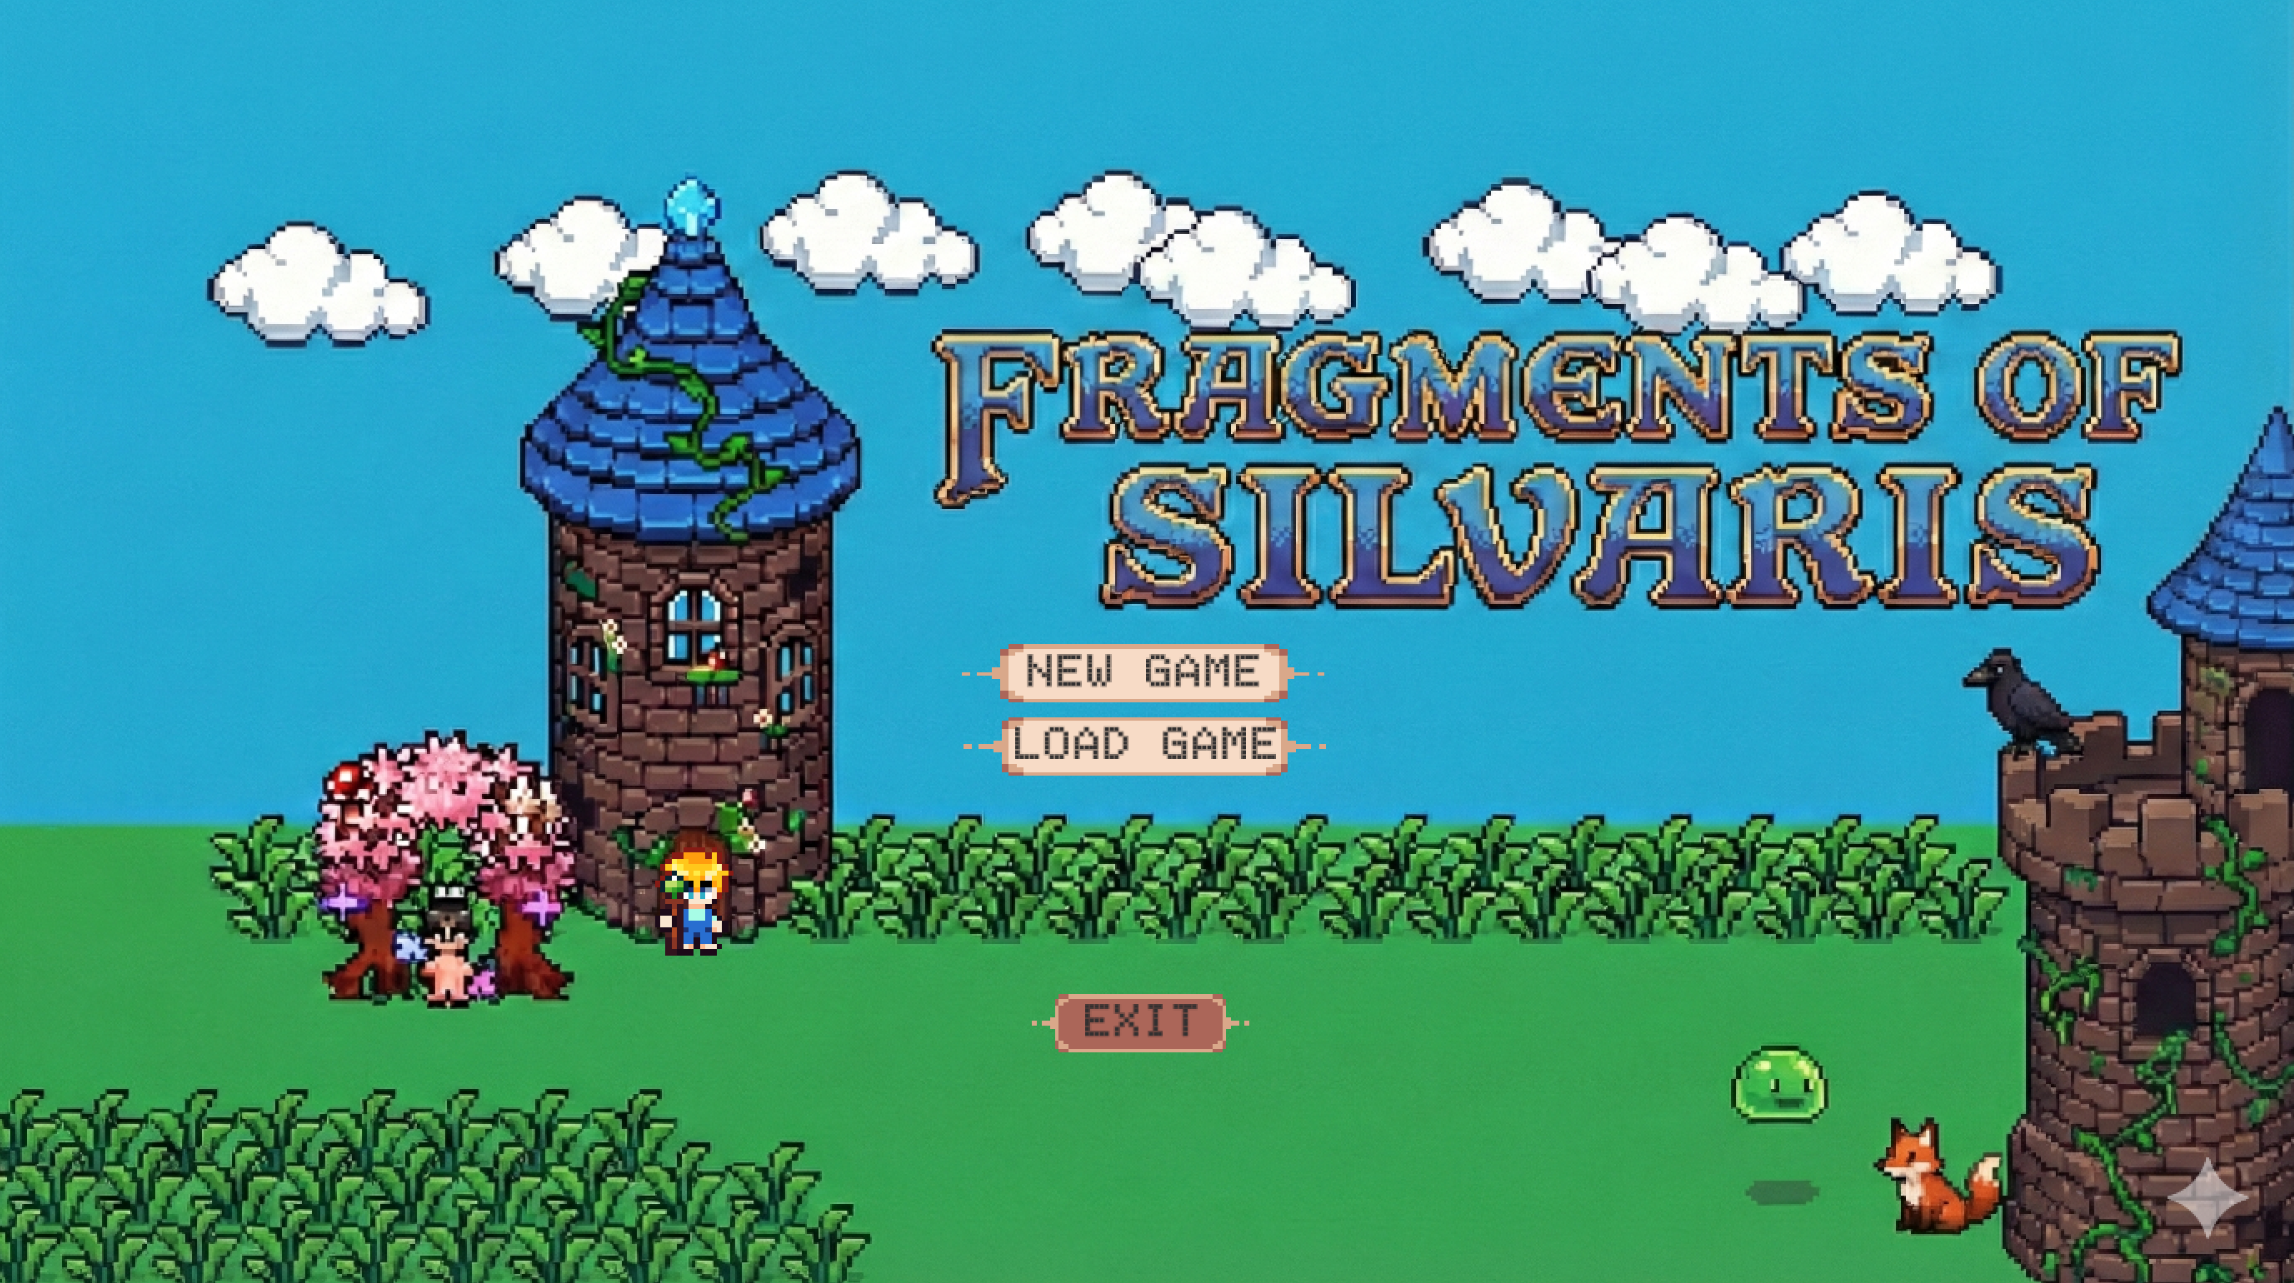
\includegraphics[width=0.8\textwidth]{Screenshot From 2026-02-11 19-06-40.png}
    \caption{Hauptmenü des Spiels}
    \label{fig:main_menu}
\end{figure}

\subsection{Spielgenre und Plattform}

Das Spiel wird als 2D Action-RPG kategorisiert und auf dem PC (Windows/Linux) ausgeführt. Es nutzt die moderne Unity 6 Engine \cite{unity_engine} mit dem Universal Render Pipeline (URP) \cite{unity_urp_2024} für optimierte Grafik-Rendering. Das Spiel läuft in Echtzeit und erfordert eine Framerate von mindestens 60 FPS für optimales Spielerlebnis.

\subsection{Zielgruppe und Setting}

Die Zielgruppe sind Spieler im Alter von 16+, die sich für klassische 2D Action-RPGs interessieren. Das Spiel spielt in einer Fantasy-Welt, in der mysteriöse Slime-Kreaturen eine Invasion führen. Der Spieler übernimmt die Rolle eines Helden, der die Aufgabe hat, diese Bedrohung zu bekämpfen.

\section{Projektziele}

Das Projektziel war die Implementierung eines funktionsfähigen 2D-RPGs mit folgenden Kernzielen:

\begin{enumerate}
    \item Implementierung eines ausgefeilten Gegner-Verhaltens mit Raycasting-basiertem Obstacle Avoidance
    \item Entwicklung eines engaging Kampfsystems mit Arc-basierte Treffererkennung
    \item Erstellung eines umfassenden RPG-Systems mit Inventar, Ausrüstung und Progression
    \item Integration von dynamischem Audio und polierter Benutzeroberfläche
    \item Dokumentation des gesamten Entwicklungsprozesses und technischer Entscheidungen
\end{enumerate}

\section{Entwicklerteam und Rollenverteilung}

Das Projekt wurde von einem Team bestehend aus vier Entwicklern umgesetzt:

\begin{itemize}
    \item \textbf{Robin Fitzek (3006199)}: 5 Scenes/Maps Design, Spiellogik und UI, Save \& Load System, Story Komponenten
    \item \textbf{Burak Yigit (3005865)}: Spiellogik, Shop System, 3 Maps/Scenes, Gold System
    \item \textbf{Aaron Seitz (3006614)}: Game Systems, Architecture, Advanced NPCs, Enemies, Player Gameplay, Inventory
    \item \textbf{Paul Weber (88487)}: NPC Systems, Ice Map Development
\end{itemize}

Entwicklungszeitraum: Oktober 2025 -- Februar 2026

% ============================================================================
% KAPITEL 2: GAMEPLAY UND MECHANIKEN
% ============================================================================

\chapter{Gameplay und Mechaniken}

\section{Kern-Spielmechaniken}

\subsection{Bewegungssteuerung}

Das Spiel unterstützt 8-direktionale Bewegung über WASD-Tasten. Der Spieler kann sich in folgende Richtungen bewegen: oben, unten, links, rechts und diagonale Richtungen (oben-links, oben-rechts, unten-links, unten-rechts). Die Animation blended zwischen den vier kardinal Richtungen basierend auf der Eingabe.

Die Bewegungsgeschwindigkeit ist konfigurierbar und wird durch Statuseffekte (Potions) beeinflusst. Der Charakter wird automatisch in die Bewegungsrichtung gedreht.

\subsection{Kampfsystem}

Das Kampfsystem basiert auf Arc-basierten Melee-Attacken, die der Spieler mit der Maus steuert. Die Attacke wird in der Richtung vom Spieler zur Mausposition durchgeführt.

\begin{itemize}
    \item \textbf{Attackenreichweite}: 2.0 Units
    \item \textbf{Angriffswinkel}: 60° Kegel (30° links + 30° rechts von der Angriffsrichtung)
    \item \textbf{Attackengeschwindigkeit}: 2 Attacken pro Sekunde (50ms Cooldown)
    \item \textbf{Multi-Target}: Kann mehrere Gegner gleichzeitig treffen
\end{itemize}

Die Treffererkennung funktioniert durch eine Kombination aus Distanzcheck und Winkelcheck:

\begin{lstlisting}[caption={Arc-basierte Treffererkennung (PlayerCombat.cs)}, label=lst:combat_arc]
void DetectAndDamageEnemiesInArc(Vector2 origin, Vector2 attackDirection)
{
    // Alle Gegner im maximalen Radius finden
    Collider2D[] potentialTargets = Physics2D.OverlapCircleAll(
        origin, attackRange, enemyLayers);

    foreach (Collider2D target in potentialTargets)
    {
        Vector2 toEnemy = (Vector2)target.transform.position - origin;
        float angleToEnemy = Vector2.Angle(attackDirection, toEnemy.normalized);

        // Gegner nur treffen wenn im Kegel
        if (angleToEnemy <= attackAngle / 2f)
        {
            target.GetComponent<EnemyHealth>()?.TakeDamage(attackDamage);
        }
    }
}
\end{lstlisting}

\subsection{Schadenssystem und Verteidigung}

Das Schadenssystem implementiert eine Defense-Formel mit abnehmenden Erträgen, um zu verhindern, dass Spieler auf hohen Leveln invincibel werden:

\begin{lstlisting}[caption={Defense-Formel mit Diminishing Returns}, label=lst:defense_formula]
float K = 20f; // Balancing-Konstante
float reduction = totalDefense / (totalDefense + K);
reduction = Mathf.Min(reduction, 0.8f); // Maximum 80% Reduktion
float damageAfterDef = Mathf.Max(damage * (1f - reduction), 1f);
\end{lstlisting}

Diese Formel stellt sicher, dass:
\begin{itemize}
    \item Erhöhte Verteidigung immer Vorteile bringt
    \item Die Steigerung aber abnehmend wird (Diminishing Returns)
    \item Spieler niemals mehr als 80% Schaden reduzieren können
    \item Minimum 1 Schaden pro Hit garantiert ist
\end{itemize}

\section{Progression und Level-Design}

\subsection{Erfahrungssystem}

Das Spiel nutzt ein exponentielles Level-Progressionssystem. Der Spieler erhält Erfahrungspunkte (XP) durch:
\begin{itemize}
    \item Besiegen von Gegnern (20 XP Base + Level-Bonus)
    \item Abschluss von Boss-Encounters
\end{itemize}

Die erforderliche XP für den nächsten Level wird exponentiell skaliert:
\begin{equation}
\text{XP}_{\text{required}} = \text{XP}_{\text{previous}} \times 1.5
\end{equation}

\subsection{Statistik-System}

Spieler-Charaktere haben folgende Statistiken:
\begin{itemize}
    \item \textbf{Gesundheit (HP)}: 100 + (Level $\times$ 10)
    \item \textbf{Mana (MP)}: 50 + (Level $\times$ 5)
    \item \textbf{Schaden (DMG)}: 10 + (Level $\times$ 2)
    \item \textbf{Verteidigung (DEF)}: Addiert von Ausrüstung
    \item \textbf{Kritische Quote}: Prozentsatz für Kritische Treffer
    \item \textbf{Kritischer Schaden}: Multiplikator für Kritische Treffer
\end{itemize}

Gegner skalieren automatisch zum Spieler-Level, um ein ausgeglichenes Kampferlebnis zu bieten.

\subsection{Level-Design und Weltenaufbau}

Das Spiel besteht aus 10 miteinander verbundenen Szenen:
\begin{itemize}
    \item 1 Hauptmenü-Szene
    \item 1 Basis-Szene (Heimat-Basis)
    \item 3 Dorf-Szenen mit NPC-Interaktionen
    \item 3 Dungeon/Wildnis-Szenen mit Gegnern
    \item 2 Boss-Arena-Szenen
\end{itemize}

Szenen sind über Trigger-Zonen miteinander verbunden und implementieren ein Spawn-Point-System für nahtlose Übergänge.

\subsubsection{Ambiente-Elemente und Sammelobjekte}

Die Spielwelt enthält verschiedene Ambiente-Elemente und Sammelobjekte, die zur Immersion und Spielmechanik beitragen:

\begin{itemize}
    \item \textbf{Tiere}: Kühe und Raben bevölkern die Landschaft und schaffen eine lebendige Spielwelt
    \item \textbf{Chests}: Versteckte Truhen in verschiedenen Szenen enthalten Story-Fragmente, die sich zu einem größeren narrativen Puzzle zusammensetzen. Das Finden aller Chests enthüllt die vollständige Hintergrundgeschichte der Welt
    \item \textbf{Vegetation}: Bäume, Blumen und Gras sorgen für visuelles Detail
\end{itemize}

\begin{figure}[H]
    \centering
    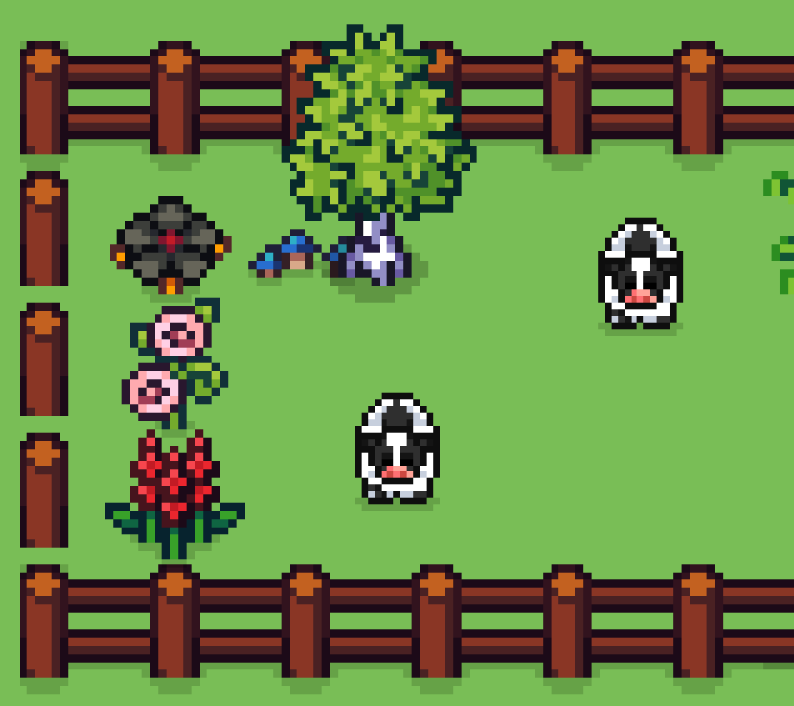
\includegraphics[width=0.6\textwidth]{Screenshot From 2026-02-11 19-12-26.png}
    \caption{Ambiente-Elemente: Kühe, Raben und Vegetation}
    \label{fig:ambient_animals}
\end{figure}

\begin{figure}[H]
    \centering
    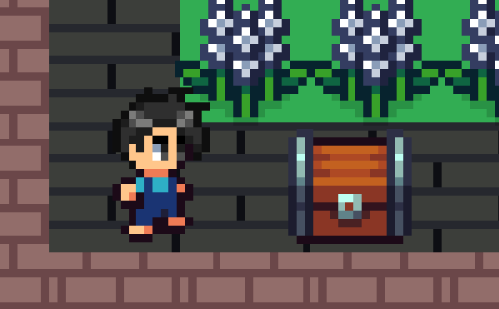
\includegraphics[width=0.4\textwidth]{Screenshot From 2026-02-11 19-16-03.png}
    \caption{Findbare Chest (Truhe) im Spiel}
    \label{fig:chest}
\end{figure}

% ============================================================================
% KAPITEL 3: STORY UND NARRATIVE
% ============================================================================

\chapter{Story und Narrative}

\section{Hintergrundgeschichte}

In einer Fantasy-Welt existiert eine alte Zivilisation mit großer magischer Macht. Durch ein mysteriöses Ritual werden slimeähnliche Kreaturen beschworen, die beginnen, die Welt zu infiltrieren. Der Spieler wird von den verbliebenen Bewohnern als Held herbeigerufen, um diese Invasion zu stoppen.

Die Geschichte wird nicht durch Zwischensequenzen, sondern durch das Journal-System erzählt.

\section{Charaktere}

\subsection{Spieler-Charakter}

Der Spieler kontrolliert einen Abenteurer, der die Mission hat, die Slime-Invasion zu stoppen. Der Charakter hat fünf verschiedene Erscheinungsformen zur Auswahl, was eine gewisse Personalisierung ermöglicht.

\begin{figure}[H]
    \centering
    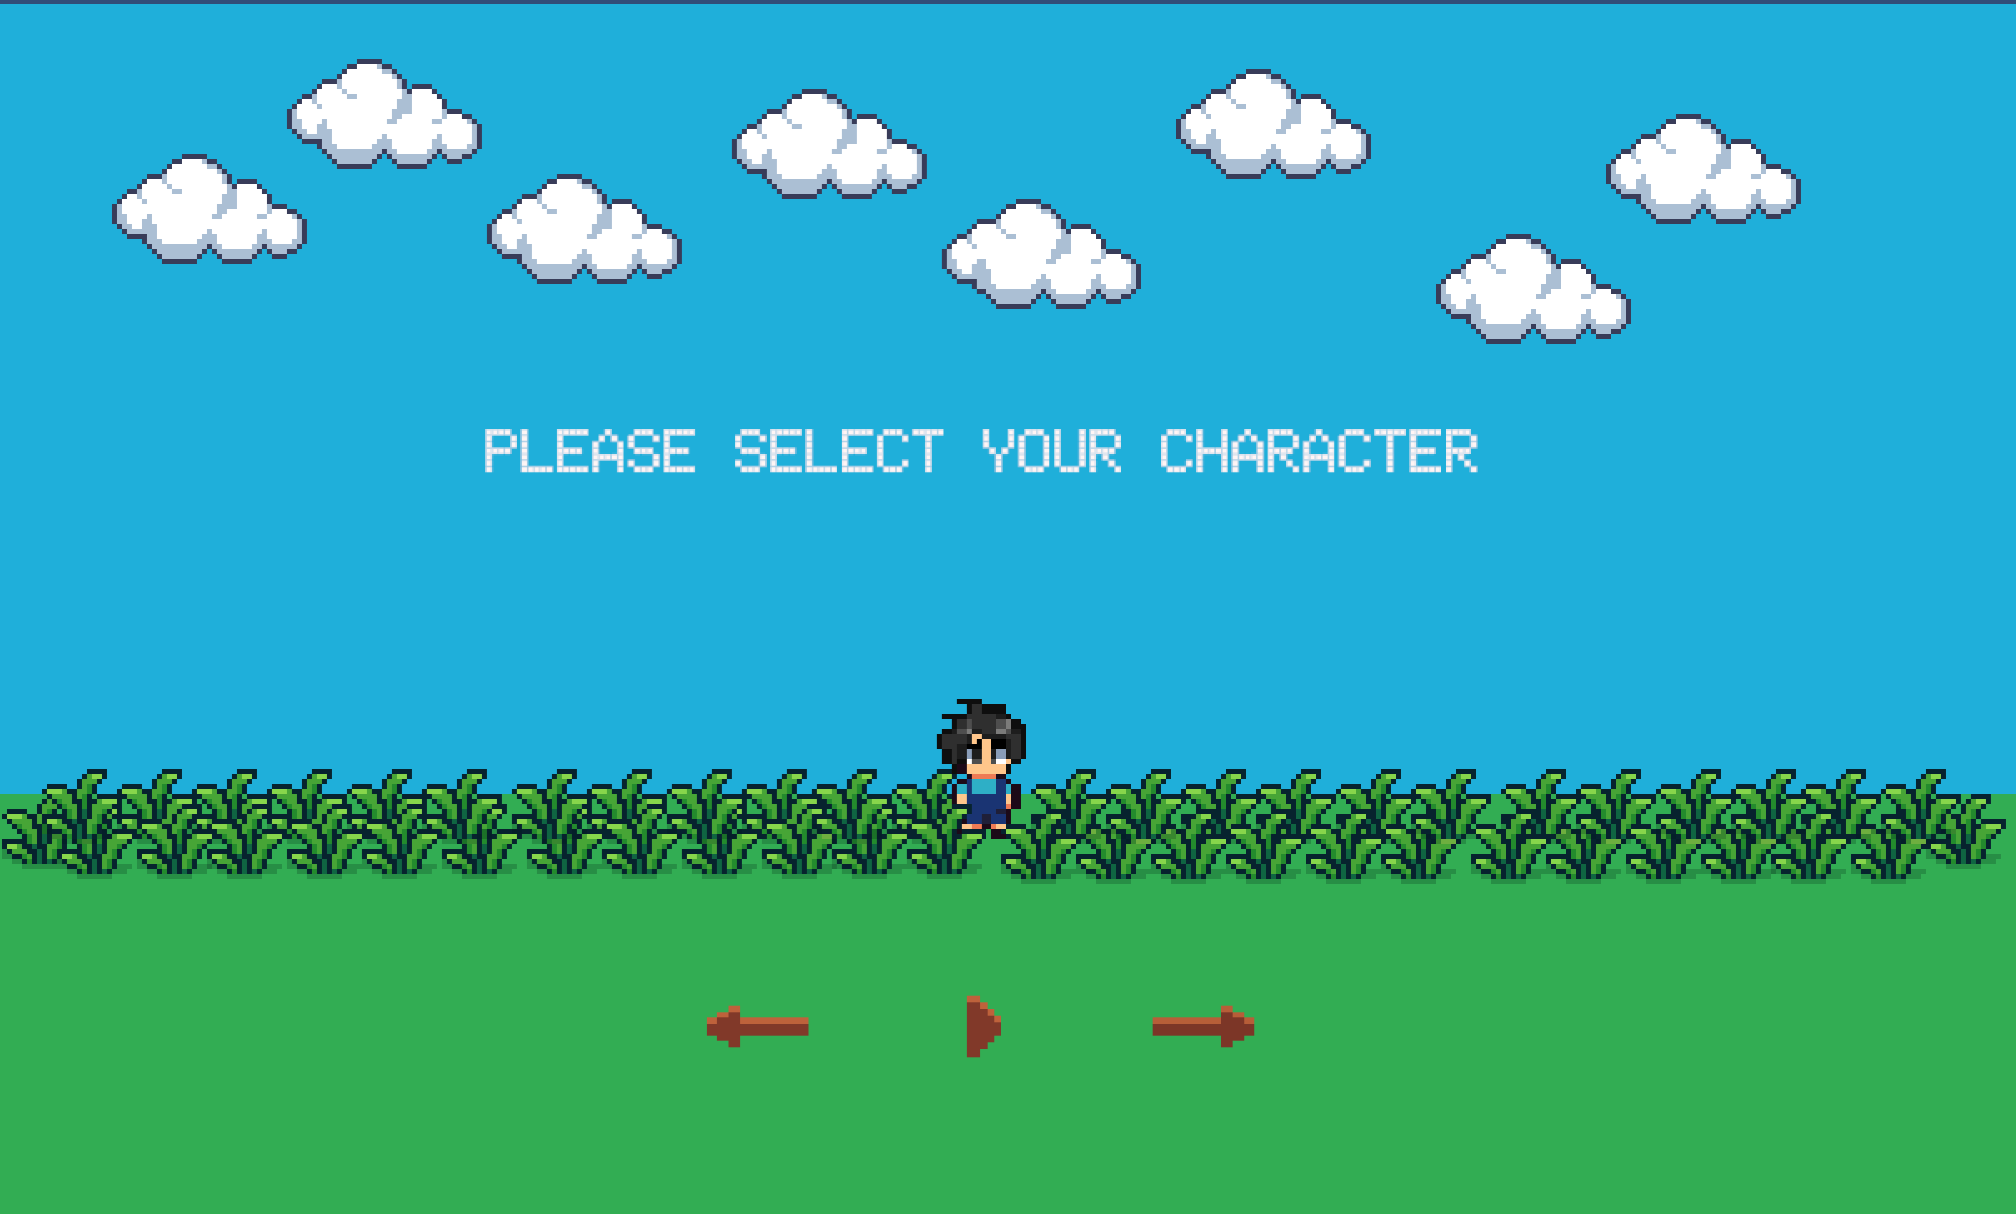
\includegraphics[width=0.7\textwidth]{Screenshot From 2026-02-11 19-07-01.png}
    \caption{Charakter-Auswahlbildschirm}
    \label{fig:character_selection}
\end{figure}

\subsection{Nicht-Spieler-Charaktere (NPCs)}

\begin{itemize}
    \item \textbf{Wandernde NPCs}: Freundliche Charaktere, die in den Dörfern herumlaufen und mit dem Spieler interagieren können
    \item \textbf{Kaufleute}: NPCs die Items verkaufen
    \item \textbf{Händler}: Spezialisierte NPCs für bestimmte Güter
\end{itemize}

\begin{figure}[H]
    \centering
    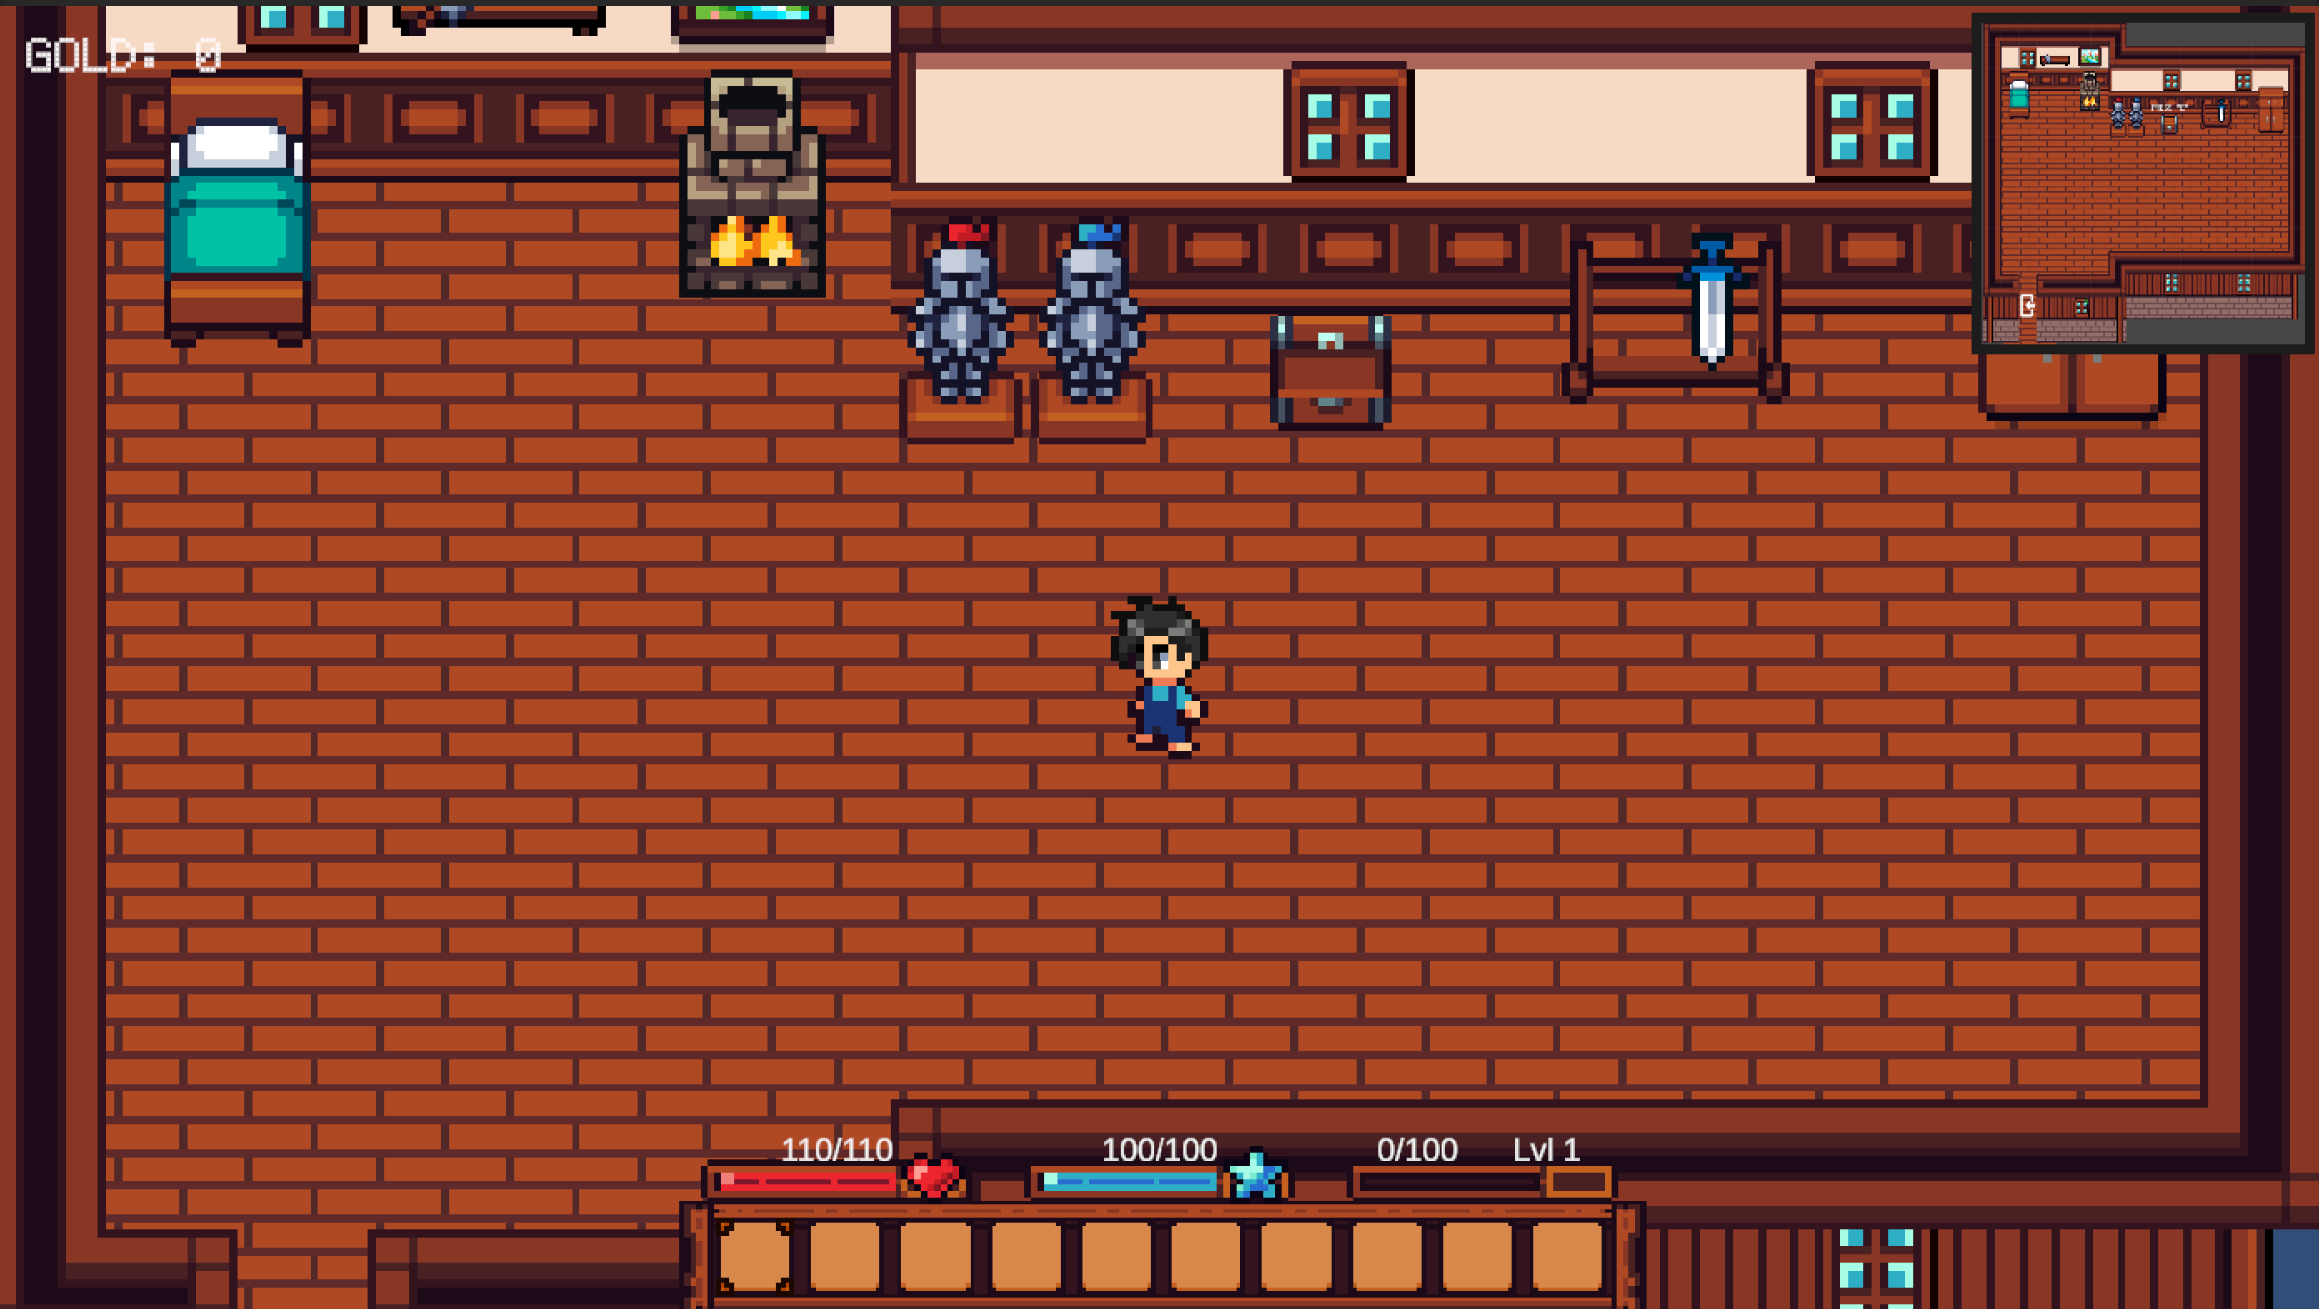
\includegraphics[width=0.6\textwidth]{Screenshot From 2026-02-11 19-10-05.png}
    \caption{NPCs in einem Gebäude}
    \label{fig:npcs_indoor}
\end{figure}

\begin{figure}[H]
    \centering
    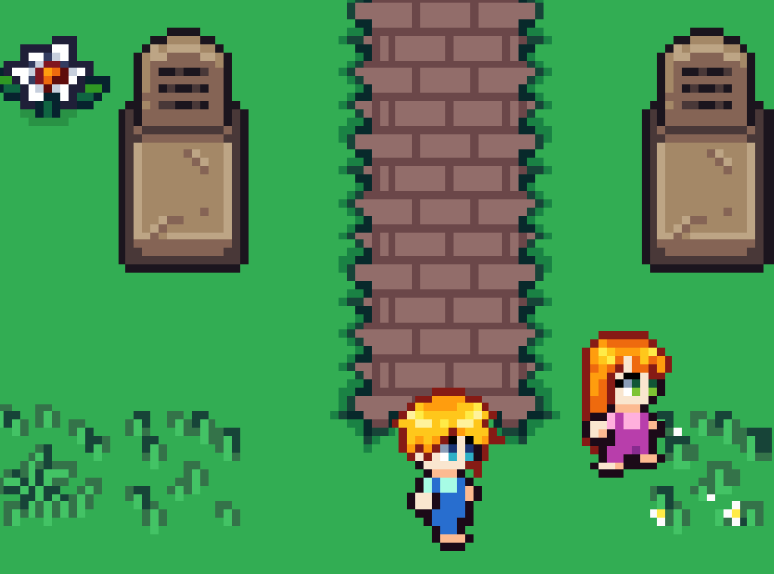
\includegraphics[width=0.6\textwidth]{Screenshot From 2026-02-11 19-11-35.png}
    \caption{Wandernde NPCs im Freien}
    \label{fig:npcs_outdoor}
\end{figure}

\subsection{Gegnerische Charaktere}

Das Spiel enthält vier Slime-Varianten als Gegner:
\begin{itemize}
    \item \textbf{Blue Slime}: Defensiv, höhere Verteidigung
    \item \textbf{Green Slime}: Standard-Gegner
    \item \textbf{Red Slime}: Aggressiv, höherer Schaden
    \item \textbf{Yellow Slime}: Schnell, höhere Geschwindigkeit
\end{itemize}

Boss-Varianten dieser Slimes spawnen mit höherem Level in Boss-Encounters.

\begin{figure}[H]
    \centering
    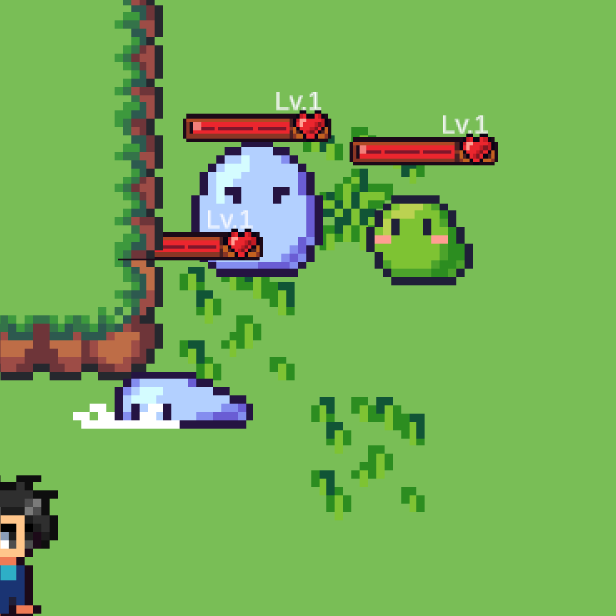
\includegraphics[width=0.5\textwidth]{Screenshot From 2026-02-11 19-11-59.png}
    \caption{Slime-Gegner mit Healthbars und Level-Anzeige}
    \label{fig:slimes}
\end{figure}

\section{Journal-System}

Das Spiel implementiert ein Journal-System, das die Geschichte erzählt und dem Spieler Hinweise gibt. Journal-Einträge werden freigeschaltet durch:
\begin{itemize}
    \item Erreichen bestimmter Szenen
    \item Besiegen bestimmter Anzahl von Gegnern
    \item Erreichen bestimmter Level-Milestones
    \item Abschluss von Boss-Encounters
\end{itemize}

Das Journal enhält über 12 Einträge und wird über eine UI-Overlay-Schnittstelle zugegriffen.

% ============================================================================
% KAPITEL 4: GRAFIK UND SOUND
% ============================================================================

\chapter{Grafik und Sound}

\section{Visueller Stil}

\subsection{Art-Style}

Das Spiel nutzt einen 2D Pixel-Art-Stil, inspiriert von klassischen RPGs wie NosTale, Terraria und The Legend of Zelda. Der Stilmix betont Gameplay gegenüber realistischer Grafik.

\subsection{Pixel-Perfect Rendering}

Das Spiel nutzt Unitys Pixel Perfect Camera Package \cite{unity_2d_pixel_perfect}, um sicherzustellen, dass Sprites pixelgenau ohne anti-aliasing gerendert werden. Dies ist essentiell für die Aufrechterhaltung der visuellen Konsistenz des Pixel-Art-Stils.

\subsection{Farbschema}

Das Farbschema variiert je nach Biom:
\begin{itemize}
    \item \textbf{Grünland}: Grüne Töne, warme Erdfarben
    \item \textbf{Dorf}: Warm und einladend
    \item \textbf{Dungeon}: Düster, mit purpurroten Tönen
    \item \textbf{Boss-Arena}: Dramatisch, kontrastig
\end{itemize}

\section{Benutzeroberflläche}

Die UI ist funktional und wird mit TextMesh Pro \cite{unity_textmesh_pro} gerendert. Zu den UI-Elementen gehören:

\begin{itemize}
    \item \textbf{Health/Mana/Stamina Bars}: Oben links, zeigt aktuelle und maximale Werte
    \item \textbf{Inventory System}: 49-Slot Grid (7x7) für Items
    \item \textbf{Equipment Screen}: 6 Ausrüstungsplätze (Waffe, Helm, Rüstung, Stiefel, Handschuhe, Accessoire)
    \item \textbf{Hotbar}: Schnellzugriff auf 10 Items
    \item \textbf{Minimap}: Kleine Karte mit Spieler-Position
    \item \textbf{Stats Sheet}: Zeigt alle Charakterstatistiken
    \item \textbf{Pause Menu}: Einstellungen, Volumenregler, Quit
    \item \textbf{Journal}: Zeigt Story-Einträge
\end{itemize}

\begin{figure}[H]
    \centering
    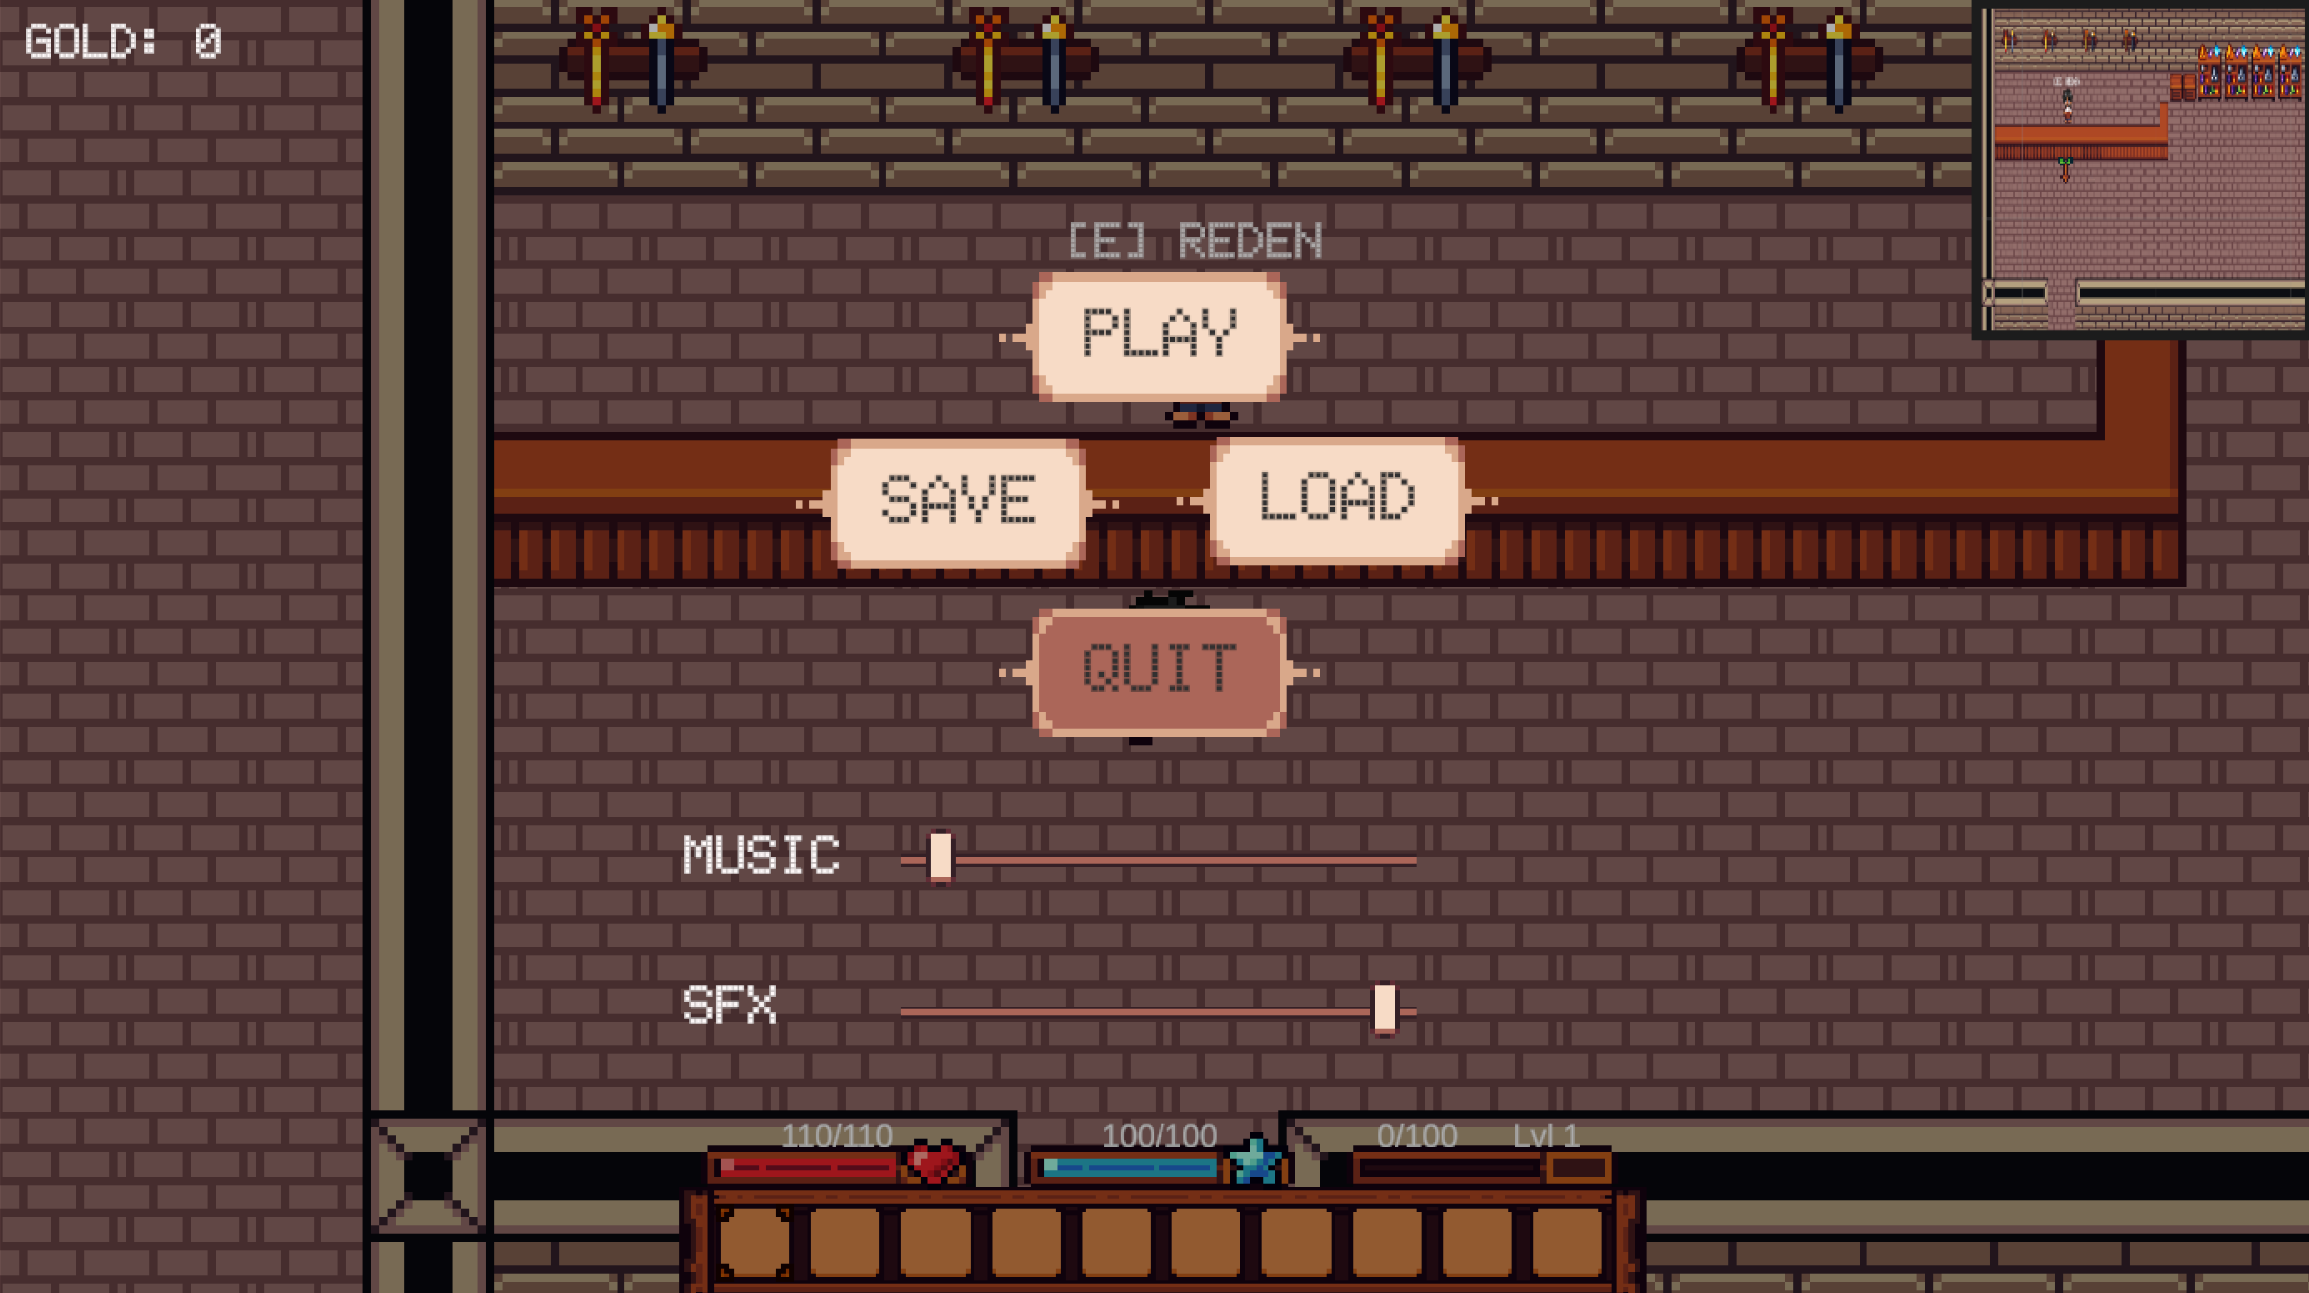
\includegraphics[width=0.7\textwidth]{Screenshot From 2026-02-11 19-16-48.png}
    \caption{Pause-Menü mit Audio-Einstellungen}
    \label{fig:pause_menu}
\end{figure}

\subsection{Minimap und Kartenansicht}

Die Minimap zeigt dem Spieler seine Position in der aktuellen Szene. Zusätzlich gibt es eine Zoom-Funktion über die Taste \textbf{M}, die eine detaillierte Übersicht der gesamten Karte bietet und dem Spieler bei der Orientierung hilft.

\begin{figure}[H]
    \centering
    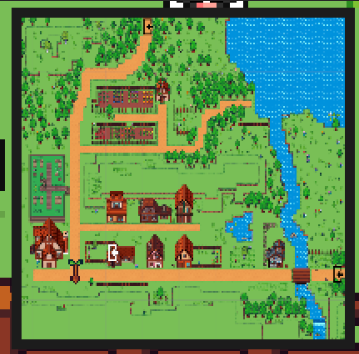
\includegraphics[width=0.3\textwidth]{Screenshot From 2026-02-11 19-11-14.png}
    \caption{Minimap-Ansicht eines Dorfgebiets}
    \label{fig:minimap_village}
\end{figure}

\begin{figure}[H]
    \centering
    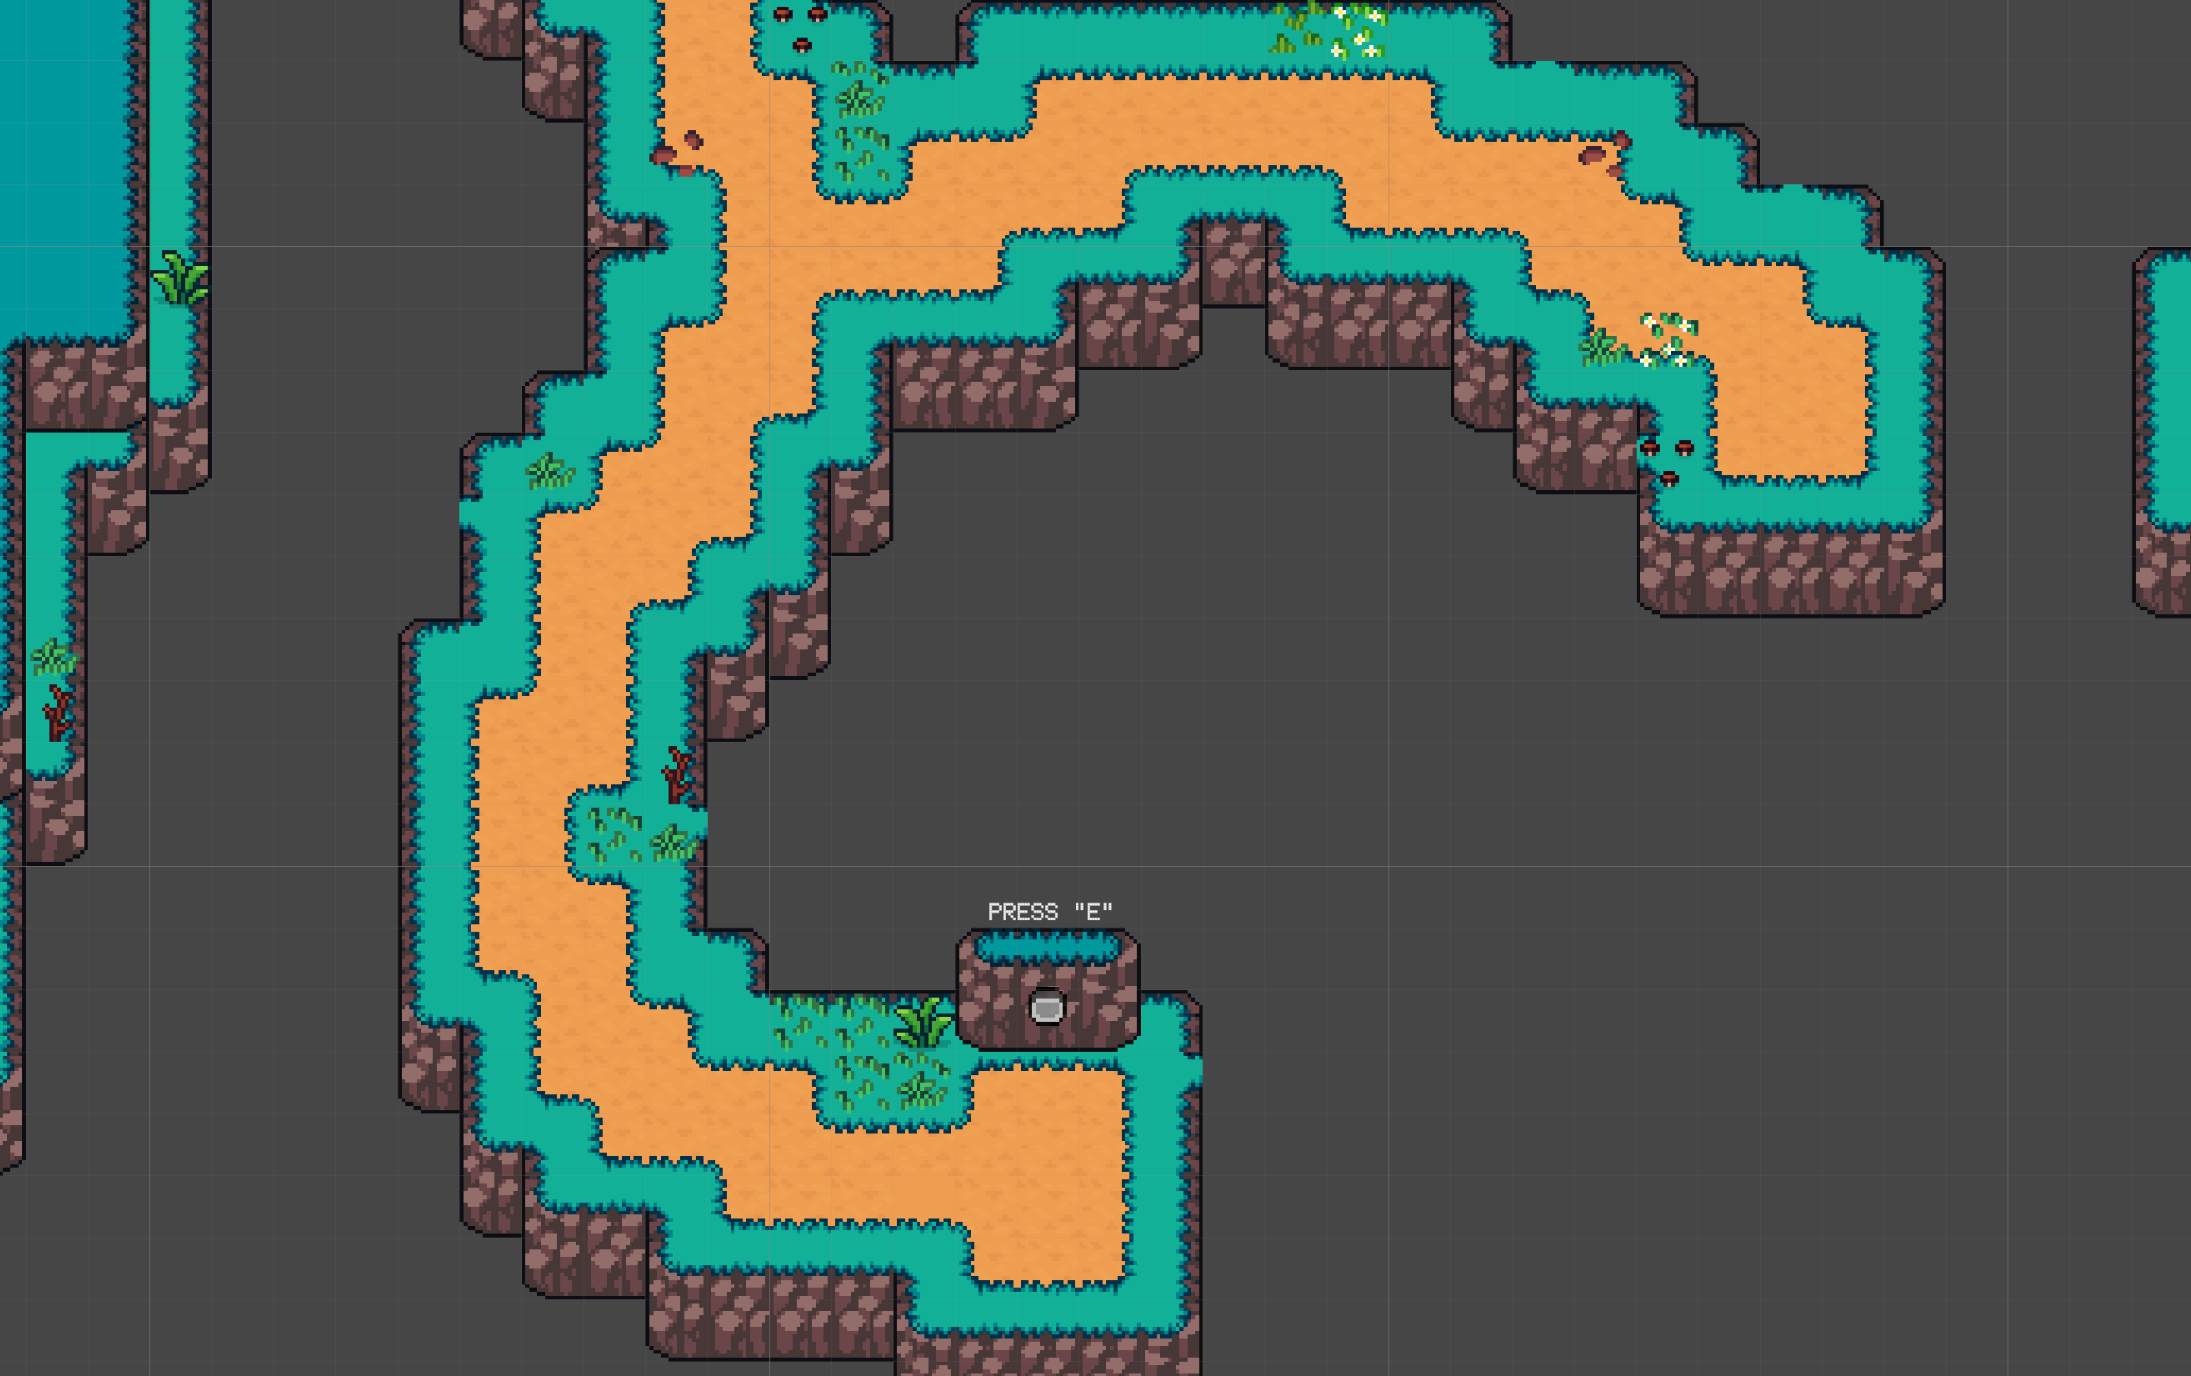
\includegraphics[width=0.7\textwidth]{Screenshot From 2026-02-11 19-21-57.png}
    \caption{Gezoomte Kartenansicht mit detaillierter Übersicht}
    \label{fig:map_zoom}
\end{figure}

\subsection{Shop- und Händler-Interface}

Das Spiel enthält ein Shop-System, über das Spieler Items kaufen und verkaufen können. Die Shop-UI zeigt verfügbare Items mit Icons und ermöglicht direkte Kaufinteraktionen.

\begin{figure}[H]
    \centering
    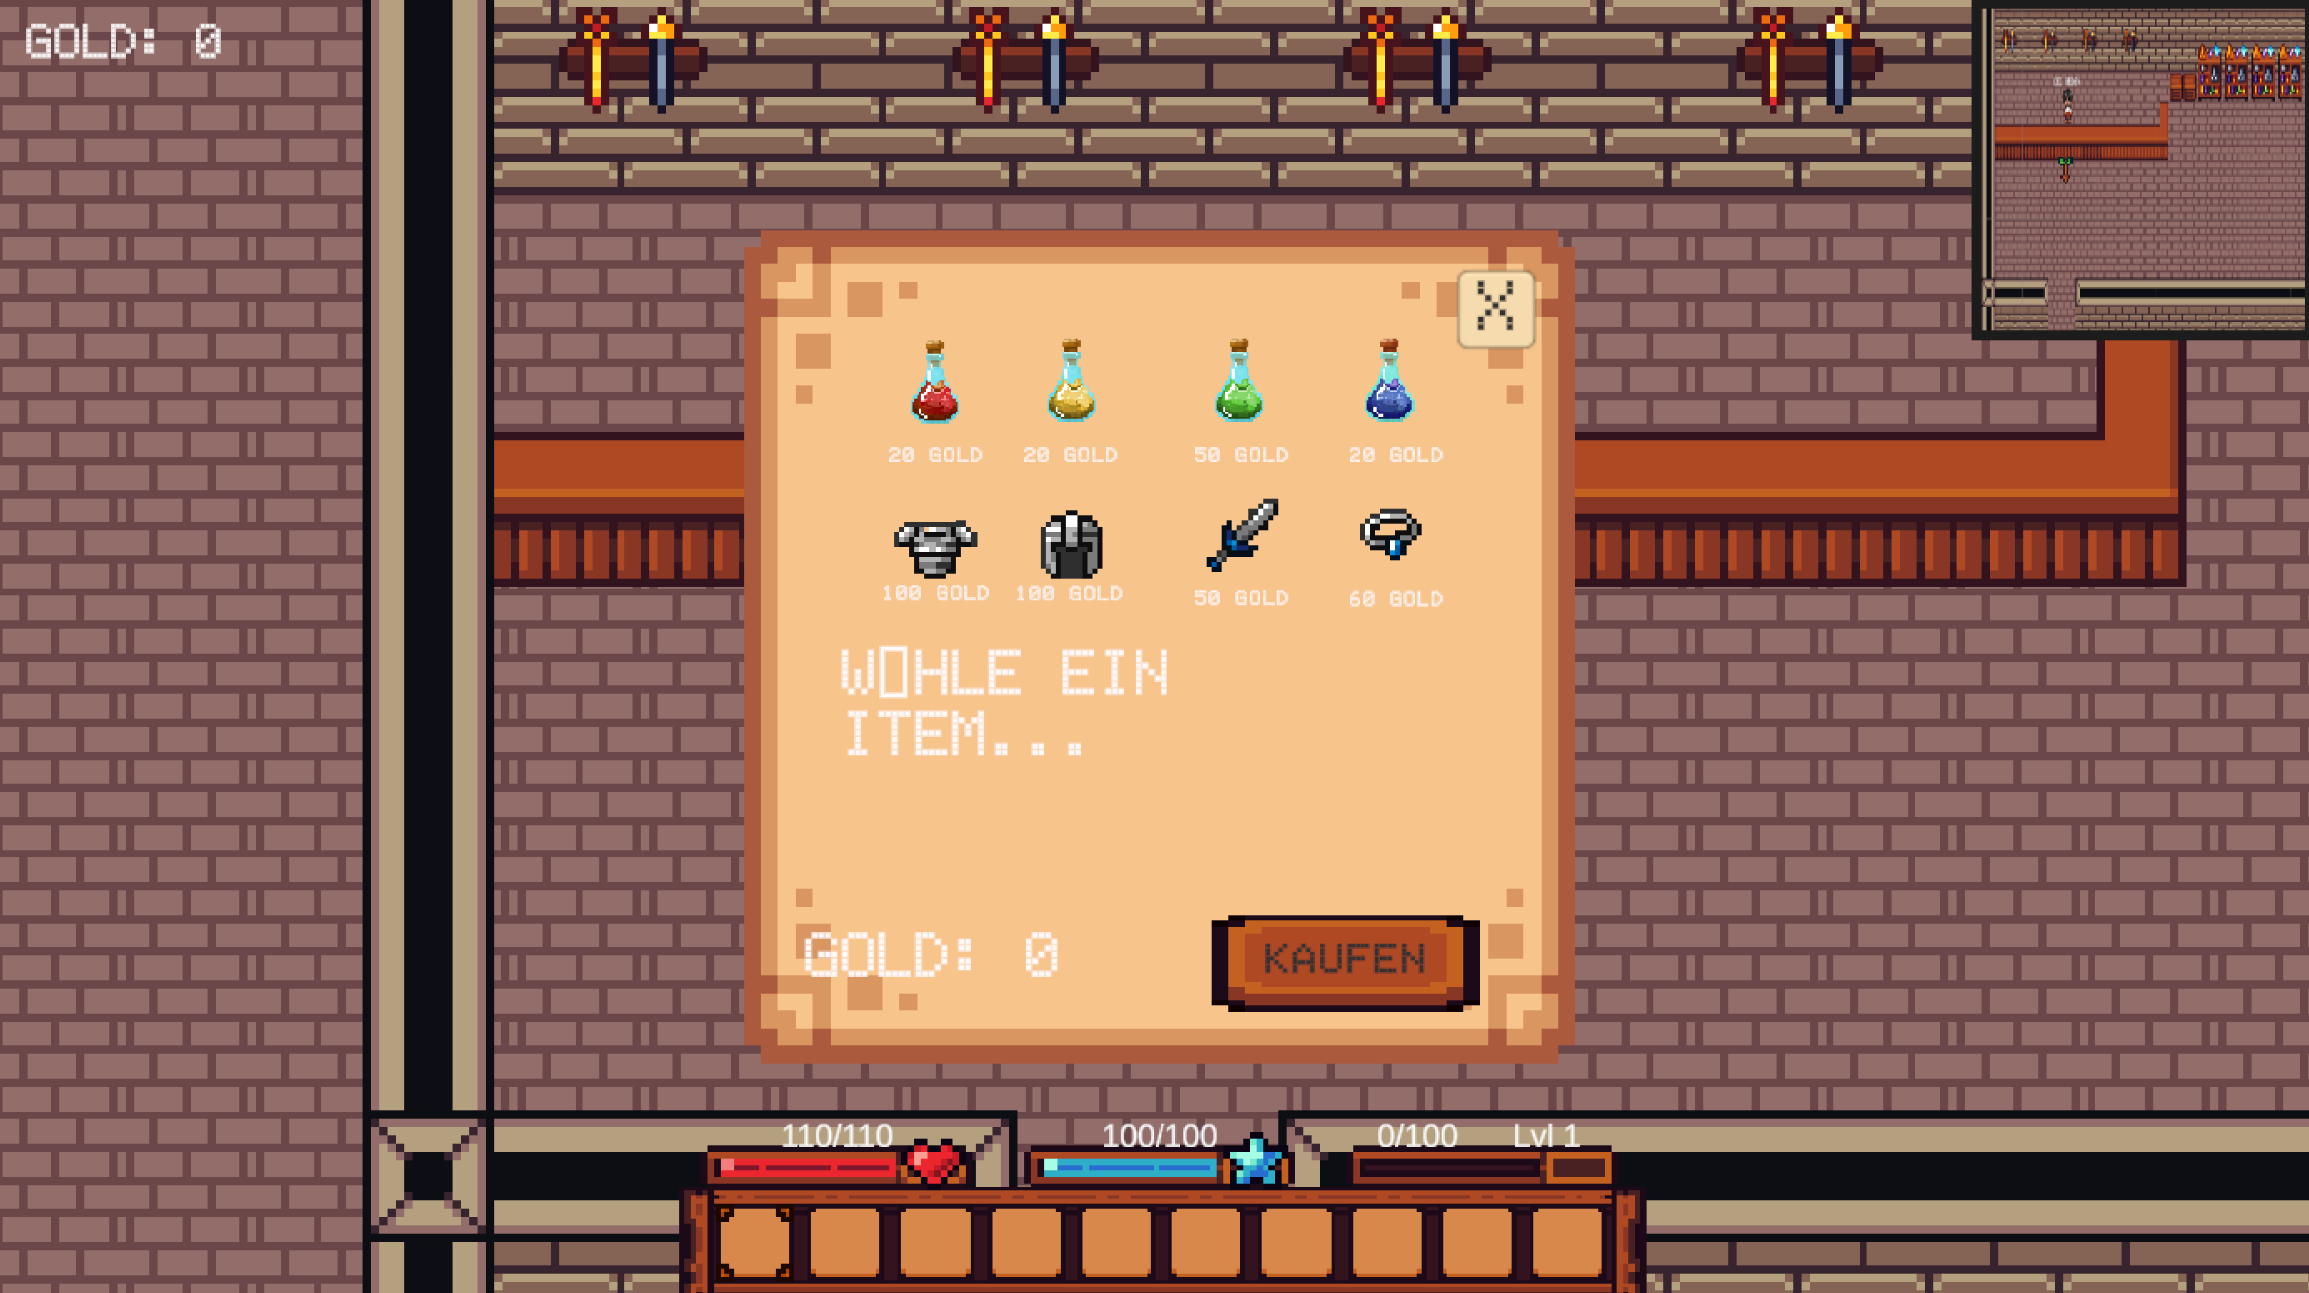
\includegraphics[width=0.7\textwidth]{Screenshot From 2026-02-11 19-17-05.png}
    \caption{Shop-Interface mit verfügbaren Items}
    \label{fig:shop_ui}
\end{figure}

\section{Sound-Design}

\subsection{Audio-Management}

Das Audio-System wird über einen zentralen AudioManager Singleton \cite{unity_engine} verwaltet, der mit dem DontDestroyOnLoad-Pattern szenenweit persistent ist.

\subsection{Musik-System}

Das Spiel implementiert ein dynamisches Musik-System mit zwei Zuständen:

\begin{itemize}
    \item \textbf{Peaceful Music}: Standard-Hintergrundmusik für Exploration
    \item \textbf{Combat Music}: Intensivere Musik wenn Gegner in Nähe sind
\end{itemize}

Das System transistioniert automatisch zwischen diesen Zuständen mit einem 1-Sekunden-Crossfade. Wenn kein Kampf für 2 Sekunden stattgefunden hat, kehrt die Musik zu Peaceful zurück.

\begin{lstlisting}[caption={Combat Music State Machine (AudioManager.cs)}, label=lst:audio_state]
public void EnterCombat()
{
    lastCombatTime = Time.time;
    if (!isInCombat)
    {
        isInCombat = true;
        StartCoroutine(CrossfadeMusic(combatMusic, 1f));
        StartCoroutine(CheckCombatEnd());
    }
}

private IEnumerator CheckCombatEnd()
{
    while (isInCombat)
    {
        if (Time.time - lastCombatTime > combatMusicDelay)
            ExitCombat();
        yield return new WaitForSeconds(0.5f);
    }
}
\end{lstlisting}

\subsection{Sound Effects}

Die Soundeffekte sind kategorisiert nach:

\begin{itemize}
    \item \textbf{Battle SFX}: Slash (Angriff), Hit (Treffer), Miss (Verfehlt), Gegner-Tod
    \item \textbf{UI SFX}: Equipment, Buy, Hover, Confirm, Deny
    \item \textbf{Shop SFX}: Shop-Open, Item-Sold, Insufficient-Gold
    \item \textbf{Movement SFX}: Footsteps (terrain-abhängig), Jump, Landing, Teleport
\end{itemize}

% ============================================================================
% KAPITEL 5: KÜNSTLICHE INTELLIGENZ
% ============================================================================

\chapter{Gegner-Verhalten und Steuerung}

Dies ist das Kernkapitel der Dokumentation, fokussiert auf das Raycasting-basierte Gegner-Verhalten.

\section{Überblick der Gegner-Systeme}

Das KI-System des Spiels besteht aus mehreren Komponenten:

\begin{enumerate}
    \item \textbf{State Machine}: 3-Zustands-Finite-State-Machine für Enemy-Verhalten
    \item \textbf{Obstacle Avoidance}: Raycasting-basiertes System zur Hindernisnavigation
    \item \textbf{Player Detection}: Proximity-basierter Erkennungsmechanismus
    \item \textbf{Combat Logic}: Angriffs-Entscheidungen mit Telegraph-System
\end{enumerate}

\section{Enemy-Bewegungs-KI}

\subsection{State Machine Architektur}

Die Enemy-KI verwendet eine 3-Zustands-Zustandsmaschine:

\begin{lstlisting}[caption={Enemy State Machine Enum}, label=lst:enemy_state]
public enum EnemyState
{
    Idle,      // Wandering, Suche nach Spieler
    Chasing,   // Verfolgung des Spielers
    Attacking  // Angriff auf den Spieler
}
\end{lstlisting}

Die Zustandsübergänge sind wie folgt definiert:

\begin{table}[h]
\centering
\caption{Gegner-Zustandsübergänge}
\label{tab:state_transitions}
\begin{tabular}{|l|l|l|}
\hline
\textbf{Von} & \textbf{Nach} & \textbf{Bedingung} \\
\hline
Idle & Chasing & \texttt{distanceToPlayer} $\leq$ 5.0 \\
Chasing & Attacking & \texttt{distanceToPlayer} $\leq$ 2.0 \\
Attacking & Chasing & \texttt{distanceToPlayer} $>$ 4.0 \\
Chasing & Idle & \texttt{distanceToPlayer} $>$ 5.0 \\
\hline
\end{tabular}
\end{table}

\subsection{Idle State -- Wandering Behavior}

Wenn kein Spieler erkannt wird, bewegt sich der Gegner in einem Wander-Muster. Das Wandering-Verhalten ist wie folgt implementiert:

\begin{enumerate}
    \item Zufälliger Ziel-Punkt wird innerhalb eines Radius um die Spawn-Position ausgewählt (standardmäßig 3 Units)
    \item Der Gegner bewegt sich zum Ziel mit der Wander-Geschwindigkeit (1 Unit/s)
    \item Bei Erreichen des Ziels: Pause für random Dauer (1-4 Sekunden)
    \item Zurück zu Schritt 1
\end{enumerate}

\begin{lstlisting}[caption={Wandering Behavior (Enemy\_Movement.cs)}, label=lst:wandering]
void HandleWandering()
{
    if (wanderPauseTimer > 0)
    {
        wanderPauseTimer -= Time.deltaTime;
        rb.linearVelocity = Vector2.zero;
        return;
    }

    if (!isWandering)
    {
        Vector2 randomOffset = Random.insideUnitCircle * wanderRadius;
        wanderTarget = spawnPosition + randomOffset;
        isWandering = true;
    }

    Vector2 direction = (wanderTarget - (Vector2)transform.position).normalized;
    direction = ApplyObstacleAvoidance(direction);
    rb.linearVelocity = direction * wanderSpeed;
}
\end{lstlisting}

Das Wandering-Verhalten nutzt auch das Obstacle Avoidance System (siehe Abschnitt 5.2.3), um Hindernisse zu vermeiden.

\subsection{Raycasting-Based Obstacle Avoidance}

\subsubsection{Motivation und Problemstellung}

Die ursprüngliche Implementierung der Enemy-Bewegung verwendete eine einfache direkte Verfolgung des Spielers. Dies führte zu folgendem Problem: \\Gegner würden in Wänden und anderen Hindernissen steckenbleiben, wenn der Spieler auf der anderen Seite eines Hindernisses war. Dies führte zu schlechtem Gameplay, da Gegner nicht intelligent um Hindernisse navigieren konnten.

Das Obstacle Avoidance System löst dieses Problem durch Multi-direktionales Raycasting, das es Gegnern ermöglicht, Hindernisse intelligente zu umgehen.

\subsubsection{Technische Implementierung}

Das System nutzt ein 3-Ray-Raycasting-System:

\begin{enumerate}
    \item \textbf{Forward Ray}: Hauptrichtung der beabsichtigten Bewegung
    \begin{itemize}
        \item Länge: 1.5 Units (raycastDistance)
        \item Winkel: 0° (direkt nach vorne)
    \end{itemize}

    \item \textbf{Left Ray}: 30° nach links rotiert
    \begin{itemize}
        \item Länge: 0.7 $\times$ raycastDistance = 1.05 Units
        \item Winkel: 30° (nach links)
    \end{itemize}

    \item \textbf{Right Ray}: 30° nach rechts rotiert
    \begin{itemize}
        \item Länge: 0.7 $\times$ raycastDistance = 1.05 Units
        \item Winkel: -30° (nach rechts)
    \end{itemize}
\end{enumerate}

Alle Raycasts werden gegen den \texttt{NPC\_Collision} Layer durchgeführt, der Wände und andere Hindernisse enthält (aber nicht den Spieler).

\subsubsection{Obstacle Avoidance Algorithmus}

Die Ausweichlogik basiert auf welche Raycasts ein Hindernis treffen:

\begin{lstlisting}[caption={Obstacle Avoidance Algorithmus (Enemy\_Movement.cs)}, label=lst:obstacle_avoid]
Vector2 ApplyObstacleAvoidance(Vector2 desiredDirection)
{
    if (obstacleLayer == 0) return desiredDirection;

    // Forward Raycast
    RaycastHit2D hit = Physics2D.Raycast(transform.position,
        desiredDirection, raycastDistance, obstacleLayer);

    if (hit.collider != null)
    {
        // Hindernis erkannt! Berechne Ausweichrichtung
        Vector2 avoidDirection = CalculateAvoidanceDirection(
            desiredDirection, hit.normal);
        return (desiredDirection + avoidDirection * avoidanceStrength)
            .normalized;
    }

    // Seitliche Raycasts
    Vector2 leftRay = RotateVector(desiredDirection, 30f);
    Vector2 rightRay = RotateVector(desiredDirection, -30f);

    RaycastHit2D hitLeft = Physics2D.Raycast(transform.position,
        leftRay, raycastDistance * 0.7f, obstacleLayer);
    RaycastHit2D hitRight = Physics2D.Raycast(transform.position,
        rightRay, raycastDistance * 0.7f, obstacleLayer);

    if (hitLeft.collider != null && hitRight.collider == null)
        return (desiredDirection + RotateVector(desiredDirection, -45f) *
            avoidanceStrength * 0.5f).normalized;
    else if (hitRight.collider != null && hitLeft.collider == null)
        return (desiredDirection + RotateVector(desiredDirection, 45f) *
            avoidanceStrength * 0.5f).normalized;
    else if (hitLeft.collider != null && hitRight.collider != null)
        return -desiredDirection;

    return desiredDirection;
}
\end{lstlisting}

Die Ausweichlogik funktioniert nach diesem Muster:

\begin{table}[h]
\centering
\caption{Obstacle Avoidance Logik nach Raycast-Ergebnissen}
\label{tab:avoidance_logic}
\begin{tabular}{|l|l|l|}
\hline
\textbf{Raycast-Treffer} & \textbf{Aktion} & \textbf{Stärke} \\
\hline
Forward Only & Seitlich ausweichen (perpendicular zur Normale) & 1.0x \\
Left Only, Right Free & Nach rechts ausweichen (-45°) & 0.5x \\
Right Only, Left Free & Nach links ausweichen (+45°) & 0.5x \\
Both Left \& Right & Umdrehen (-180°) & 1.0x \\
None & Keine Ausweichung & -- \\
\hline
\end{tabular}
\end{table}

\subsubsection{Smoothing und Performance}

Um jittery Movement zu vermeiden, implementiert das System:

\begin{itemize}
    \item \textbf{Cooldown System}: 0.2 Sekunden Cooldown zwischen Ausweichentscheidungen
    \item \textbf{Direction Caching}: Die letzte Ausweichrichtung wird cached für sanfte Übergänge
    \item \textbf{Weighted Blending}: Gewichtete Kombination von Bewegungs- und Ausweichrichtung
\end{itemize}

Die Performance-Auswirkung von Raycasting ist minimal, da nur 3 Raycasts pro Frame durchgeführt werden (mit 0.2s Cooldown reduziert sich dies auf etwa 15 Raycasts pro Sekunde pro Enemy).

\subsection{Chasing State -- Player Pursuit}

Wenn der Spieler erkannt wird (Distanz $\leq$ detectionRange), betritt der Gegner den Chasing State. In diesem State:

\begin{enumerate}
    \item Die Richtung zum Spieler wird jedes Frame berechnet
    \item Das Obstacle Avoidance System wird angewendet
    \item Der Gegner bewegt sich mit speed (2 Units/s) in diese Richtung
    \item Der Gegner wendet sich dem Spieler zu (Sprite-Flipping basierend auf Richtung)
    \item Audio-Manager wird informiert (Combat Music startet)
\end{enumerate}

\section{Angriffs-Logik}

\subsection{Attack Telegraph System}

Ein zentrales Feature der Combat-Mechanik ist das Attack Telegraph System. Dies ermöglicht es dem Spieler, Gegner-Angriffe zu antizipieren und auszuweichen.

\subsubsection{Motivation}

In frühen Spielversionen führten Gegner Angriffe ladezeit durch. Dies führte zu Spieler-Frustration, da keine Reaktionsmöglichkeit existierte. Das Telegraph System löst dies durch eine "Vorwarnungszeit" vor dem eigentlichen Schaden.

\subsubsection{Parameter}

\begin{table}[h]
\centering
\caption{Attack Telegraph Parameter}
\label{tab:attack_params}
\begin{tabular}{|l|l|l|}
\hline
\textbf{Parameter} & \textbf{Wert} & \textbf{Beschreibung} \\
\hline
\texttt{attackRange} & 2.0 Units & Entfernung für Angriffsentscheidung \\
\texttt{attackHitRange} & 1.0 Units & Tatsächliche Trefferreichweite \\
\texttt{attackWindupTime} & 0.4 Sekunden & Telegraph-Zeit \\
\texttt{attackCooldown} & 1.5 Sekunden & Cooldown zwischen Angriffen \\
\hline
\end{tabular}
\end{table}

Beachte, dass \texttt{attackRange} $>$ \texttt{attackHitRange}. Dies bedeutet:
\begin{itemize}
    \item Gegner beginnen Angriff bei 2.0 Units Distanz
    \item Aber Schaden wird nur angewendet wenn Spieler bei 1.0 Units ist
    \item Dies ermöglicht Spieler, während des Wind-ups auszuweichen
\end{itemize}

\subsubsection{Attack Sequence}

Eine Angriff läuft wie folgt ab:

\begin{enumerate}
    \item Gegner-Distanz $\leq$ attackRange → Attacking State
    \item Attack Animation wird gestartet
    \item Wind-up Zeit (0.4s) -- \textbf{Spieler kann ausweichen!}
    \item Nach Wind-up: Prüfe ob Spieler noch in attackHitRange
    \item IF YES: Schaden anwenden | IF NO: Angriff verfehlt
    \item Cooldown warten (1.5s)
    \item Zurück zu Schritt 1
\end{enumerate}

\begin{lstlisting}[caption={Attack mit Wind-up (Enemy\_Movement.cs)}, label=lst:attack_windup]
IEnumerator AttackWithWindup()
{
    isAttacking = true;
    anim.SetTrigger("Attack");

    // Wind-up Zeit - Spieler kann ausweichen!
    yield return new WaitForSeconds(attackWindupTime);

    // NOW: Check if player still in range
    if (player != null)
    {
        float currentDistance = Vector2.Distance(
            transform.position, player.position);

        if (currentDistance <= attackHitRange)
        {
            PlayerStats playerStats = player
                .GetComponent<PlayerStats>();
            if (playerStats != null)
                playerStats.TakeDamage(attackDamage);
        }
    }

    yield return new WaitForSeconds(0.3f);
    isAttacking = false;
}
\end{lstlisting}

\subsection{Contact Damage}

Zusätzlich zu Angriff-basierten Schaden können Gegner auch durch Kontakt Schaden verursachen (separate Collision-basierte Schaden). Dies ist implementiert über einen OnCollisionStay-Callback, der regelmäßig (etwa 1x pro Sekunde) Schaden anwendet.

\section{Weitere KI-Features}

\subsection{NPC Wandering}

Freundliche NPCs nutzen ein ähnliches Wandering-System wie Gegner im Idle State. Allerdings haben sie unterschiedliche Konfigurationen:
\begin{itemize}
    \item Größere wanderRadius (bis zu 10 Units)
    \item Längere Pausen zwischen Bewegungen
    \item Keine Raycasting-Hinderniserkennung (einfacher)
\end{itemize}

\subsection{Boss Wave System}

Boss-Encounters verwenden ein Wave-basiertes System (SlimeWaveController). Charakteristiken:
\begin{itemize}
    \item Ziel: 60 Slimes besiegen
    \item Spieler kontrolliert Spawn-Rate über Buttons
    \item Automatisches Fallback: 2 Slimes alle 60 Sekunden (wenn Spieler nichts macht)
    \item Boss-Slimes spawnen mit \texttt{playerLevel + 3} für Herausforderung
    \item Journal-Einträge entsperren bei 20, 40, 60 Kills
\end{itemize}

% ============================================================================
% KAPITEL 6: TECHNISCHE IMPLEMENTIERUNG
% ============================================================================

\chapter{Technische Implementierung}

\section{Game Engine und Tools}

\subsection{Unity Engine}

Das Spiel wurde in \textbf{Unity 6000.2.7f2} \cite{unity_engine} entwickelt, der neuesten LTS-Version von Unity. Die Wahl von Unity war strategisch:

\begin{itemize}
    \item Für 2D-Spiele optimiert
    \item Schnelle Iteration und Playtesting
    \item Großer Asset Store für vorgefertigte Komponenten
    \item Starke C\# Integration mit modernem Tooling
\end{itemize}

\subsection{Universal Render Pipeline (URP)}

Das Projekt nutzt \ac{URP} 17.2.0 \cite{unity_urp_2024} für Grafik-Rendering. \ac{URP} ist ein skriptbarer Rendering-Pipeline, der Flexibilität und Performance bietet.

\subsection{Key Packages}

Folgende wichtige Packages wurden integriert:

\begin{table}[h]
\centering
\caption{Unity Packages und Versionen}
\label{tab:unity_packages}
\begin{tabular}{|l|l|l|}
\hline
\textbf{Package} & \textbf{Version} & \textbf{Verwendung} \\
\hline
2D Animation & 12.0.2 & Sprite-Rigging und Skelettanimation \\
Pixel Perfect & 5.1.1 & Pixel-perfektes Rendering \\
Input System & 1.14.2 & Moderne Input-Verarbeitung \\
Cinemachine & 3.1.4 & Kamera-Kontrolle \\
\hline
\end{tabular}
\end{table}

\section{Code-Architektur}

\subsection{Singleton Pattern}

Das Spiel nutzt das Singleton Pattern für Manager-Klassen, die global zugegriffen werden müssen:

\begin{itemize}
    \item \textbf{AudioManager}: Zentrale Audio-Verwaltung
    \item \textbf{SaveManager}: Speichern/Laden von Spielzustand
    \item \textbf{SceneTransitionManager}: Szenen-Übergänge mit Spawn Points
    \item \textbf{GoldManager}: Währungs-Management
    \item \textbf{NotificationManager}: Toast-Benachrichtigungen
\end{itemize}

Das Singleton Pattern wird mit dem DontDestroyOnLoad-Ansatz implementiert:

\begin{lstlisting}[caption={Singleton Pattern Implementierung}, label=lst:singleton]
public class AudioManager : MonoBehaviour
{
    public static AudioManager Instance { get; private set; }

    private void Awake()
    {
        if (Instance == null)
        {
            Instance = this;
            DontDestroyOnLoad(gameObject);
        }
        else
        {
            Destroy(gameObject);
        }
    }
}
\end{lstlisting}

Vorteile:
\begin{itemize}
    \item Globaler Zugriff auf wichtige Manager
    \item Persistenz über Szenen-Grenzen hinweg
    \item Verhindert Duplikate durch Pattern-Implementierung
\end{itemize}

\subsection{Event-Driven Architecture}

Das Spiel nutzt C\# Events für lose Kopplung zwischen Systemen. Beispiel: Wenn sich Player-Stats ändern, werden diese über Events kommuniziert:

\begin{lstlisting}[caption={Event-Driven Architecture Beispiel}, label=lst:event_driven]
public class PlayerStats : MonoBehaviour
{
    public event Action OnHealthChanged;
    public event Action OnLevelUp;
    public event Action<int, int> OnLevelUpWithLevel;

    public void TakeDamage(float damage)
    {
        health -= damage;
        OnHealthChanged?.Invoke();
    }
}

public class PlayerResourceBarsUI : MonoBehaviour
{
    private void Start()
    {
        PlayerStats stats = player.GetComponent<PlayerStats>();
        stats.OnHealthChanged += UpdateHealthBar;
    }
}
\end{lstlisting}

Vorteile:
\begin{itemize}
    \item Lose Kopplung zwischen Systems
    \item UI aktualisiert automatisch bei Stat-Änderungen
    \item Leicht erweiterbar für neue Listener
\end{itemize}

\subsection{Inventory System (MVC Pattern)}

Das Inventory System implementiert ein MVC-ähnliches Pattern:

\begin{itemize}
    \item \textbf{Model} (Inventory.cs): 49-Slot-Datenstruktur, Item-Verwaltung
    \item \textbf{Controller} (PlayerInventory.cs): Geschäftslogik, Add/Remove Items
    \item \textbf{View} (InventorySlotUI.cs): UI-Darstellung, Drag-and-Drop
\end{itemize}

Das System nutzt Scriptable Objects für Item-Daten:

\begin{itemize}
    \item Jedes Item hat eine ItemData ScriptableObject-Definition
    \item ID-basiertes Lookup ermöglicht Serialisierung (ScriptableObjects sind nicht serialisierbar)
    \item 49 Slots können stackable (potions) oder non-stackable (equipment) Items halten
\end{itemize}

\subsection{Scene Management}

Das Spiel implementiert ein Scene Transition System mit nahtlosen Übergängen:

\begin{enumerate}
    \item Spieler betritt Trigger Zone (SceneTrigger.cs)
    \item Loading Screen wird angezeigt (mit UI in unscaled Time)
    \item Szene wird asynchron geladen
    \item SpawnPoint-System teleportiert Spieler zu korrekter Position
    \item Loading Screen faded aus
\end{enumerate}

Die Spawn Point Architektur ermöglicht es, mehrere Einstiegspunkte pro Szene zu haben (z.B. unterschiedliche Türen/Portale).

\subsection{Save/Load System}

Das Spiel nutzt ein Hybrid Save-System:

\begin{itemize}
    \item \textbf{PlayerPrefs}: Einfache Daten (Lautstärke, Einstellungen)
    \item \textbf{JSON Files}: Komplexe Daten (Inventory, Stats, Position)
    \item \textbf{SceneData}: World-State persistent über SaveManager
\end{itemize}

Das Hauptproblem war die Serialisierung von ScriptableObject-Referenzen. Lösung: ID-basiertes Item-Lookup.

\section{Performance-Optimierungen}

\subsection{Culling-System}

Das CullingOptimizer Script deaktiviert Renderer für Objekte außerhalb der Camera View:

\begin{itemize}
    \item Distance-based Culling mit konfigurierbarem Radius
    \item Signifikanter FPS-Boost in großen Szenen
    \item Automatisches Re-enabling wenn Objekt in Nähe kommt
\end{itemize}

\subsection{Animator Culling}

AnimatorCulling Script reduziert Animation Updates für Off-screen Objects:

\begin{itemize}
    \item Three Culling Modes: Always Animate, Cull Update Transforms, Cull Completely
    \item Massive Reduktion von CPU-Last bei vielen Enemies
    \item Spieler bemerkt keinen visuellen Unterschied
\end{itemize}

\subsection{Dynamic Quality}

PerformanceOptimizer überwacht FPS und reduziert Quality bei Bedarf:

\begin{itemize}
    \item Targets: 60 FPS
    \item Bei Unterschreitung: Particle Effects reduzieren, Shadow Quality senken, etc.
    \item Dynamisches Adjustment ohne Game-Pause
\end{itemize}

% ============================================================================
% KAPITEL 7: ENTWICKLUNGSPROZESS
% ============================================================================

\chapter{Entwicklungsprozess}

\section{Planung und Projektmanagement}

\subsection{Entwicklungsphasen}

Das Projekt wurde in 5 Phasen über ca. 6 Monate entwickelt:

\begin{description}
    \item[Phase 1 (Oct 2025)]: \textbf{Core Mechanics}
    \begin{itemize}
        \item Movement System, Basic Combat, Player Sprites
        \item UI Grundlagen (Health Bar, Inventory)
    \end{itemize}

    \item[Phase 2 (Nov 2025)]: \textbf{Gegner-Verhalten \& Raycasting}
    \begin{itemize}
        \item Raycasting-basiertes Obstacle Avoidance implementieren
        \item State Machine für Enemies
        \item Combat Music System
    \end{itemize}

    \item[Phase 3 (Dec 2025)]: \textbf{RPG Systems}
    \begin{itemize}
        \item Inventory System mit Equipment
        \item Level-Progression und Stat-Scaling
        \item Save/Load System
    \end{itemize}

    \item[Phase 4 (Jan 2026)]: \textbf{Polish \& Audio}
    \begin{itemize}
        \item Sound Design und Music Integration
        \item UI Polish, Feedback-Systeme
        \item Performance Optimizations
    \end{itemize}

    \item[Phase 5 (Feb 2026)]: \textbf{Boss Encounter \& Testing}
    \begin{itemize}
        \item Boss Wave System implementieren
        \item Playtesting und Bug Fixing
        \item Final Polish und Documentation
    \end{itemize}
\end{description}

\subsection{Versionskontrolle}

Das Projekt nutzte Git \cite{nostalelike_github_repo} mit GitHub für Versionskontrolle:

\begin{itemize}
    \item \textbf{Main Branch}: Stabiler, produktionsreifer Code
    \item \textbf{Develop Branch}: Integrationsbranch für Features
    \item \textbf{Feature Branches}: Isolierte Feature-Entwicklung
    \item \textbf{80+ Commits}: Regelmäßiges Commitment mit beschreibenden Nachrichten
\end{itemize}

\section{Meilensteine und Deliverables}

\begin{itemize}
    \item \textbf{Oct 2025}: First Playable Demo mit Basic Movement + Combat
    \item \textbf{Nov 2025}: Gegner-Verhalten mit Raycasting funktionsfähig
    \item \textbf{Dec 2025}: Inventory System functional und Save/Load arbeitet
    \item \textbf{Jan 2026}: Audio System integrated, Sound Effects komplett
    \item \textbf{Feb 2026}: Boss Encounter spielbar, Game Loop geschlossen
\end{itemize}

\section{Testing und Quality Assurance}

\subsection{Testing-Strategien}

\begin{enumerate}
    \item \textbf{Manual Playtesting}: Team-Mitglieder spielen regelmäßig das Spiel
    \item \textbf{Debug Logging}: Debug.Log Statements in kritischen Code-Pfaden
    \item \textbf{Unity Gizmos}: Visuelle Debugging von Erkennungsreichweiten und Raycasts
    \item \textbf{Automated Checks}: Compile-time Checks, Unity's Scene validation
\end{enumerate}

\subsection{Bug Tracking}

Bugs wurden über GitHub Issues verfolgt, mit Labels nach Kategorie:
\begin{itemize}
    \item \texttt{bug}: Tatsächliche Fehler
    \item \texttt{enhancement}: Verbesserungen vorhandener Features
    \item \texttt{gameplay}: Balancing und Design Issues
    \item \texttt{performance}: Optimierungs-Gelegenheiten
\end{itemize}

\section{Herausforderungen und Lösungen}

\subsection{Challenge 1: Enemy Pathfinding}

\begin{description}
    \item[Problem] Enemies würden in Wänden steckenbleiben, wenn der Spieler dahinter war. Dadurch entstand schlechtes Gameplay-Gefühl.
    \item[Ansätze]
    \begin{enumerate}
        \item Erste Idee: A* Pathfinding -- zu komplex, keine NavMesh vorhanden
        \item Zweite Idee: Simple Avoid-Walls -- funktioniert nicht gut mit komplexen Geometrien
        \item Dritte Idee (implementiert): Multi-directional Raycasting
    \end{enumerate}
    \item[Lösung] Raycasting-System mit 3 Rays (forward, left 30°, right 30°) mit dynamischer Ausweichlogik
    \item[Resultat] Enemies navigieren natürlich um Hindernisse, ohne Complex Pathfinding
\end{description}

\subsection{Challenge 2: Scene Persistence}

\begin{description}
    \item[Problem] Spieler-Position wurde nach Scene-Load zurückgesetzt. Außerdem spawn mehrere Manager-Instanzen bei jedem Scene-Load.
    \item[Lösung]
    \begin{itemize}
        \item SpawnPoint-System: Named spawn locations in jeder Szene
        \item SceneTransitionManager verwaltet target spawn point
        \item Singleton Pattern mit frühen Instance-Checks verhindert Duplikate
    \end{itemize}
    \item[Resultat] Nahtlose Scene-Übergänge, kein Gameobject-Spam
\end{description}

\subsection{Challenge 3: Combat Feel}

\begin{description}
    \item[Problem] Angriffe fühlten sich instant und unfair an. Spieler konnte nicht auf Gegner-Angriffe reagieren.
    \item[Lösung]
    \begin{itemize}
        \item Attack Telegraph System: 0.4s Wind-up vor Schaden
        \item Smaller Hit Range (1.0 Units) vs Larger Attack Range (2.0 Units)
        \item Sound- und Visual Feedback
    \end{itemize}
    \item[Resultat] Skill-basiertes Combat mit Ausweich-Möglichkeiten
\end{description}

\subsection{Challenge 4: Inventory Serialisierung}

\begin{description}
    \item[Problem] ScriptableObject-Referenzen können nicht direkt JSON-serialisiert werden.
    \item[Lösung] ID-basiertes Lookup System:
    \begin{itemize}
        \item Jedes Item hat eine eindeutige String-ID
        \item Save speichert nur Item-IDs und Mengen
        \item Load rekonstruiert Items via Lookup-Dictionary
    \end{itemize}
    \item[Resultat] Robustes Save/Load System ohne Data Corruption
\end{description}

\subsection{Challenge 5: Defense Scaling}

\begin{description}
    \item[Problem] Bei hohen Leveln wird lineare Defense Formel unausgeglichen. Spieler werden invincibel.
    \item[Lösung] Diminishing Returns Formel:
    \begin{equation}
        \text{reduction} = \min\left(\frac{\text{defense}}{\text{defense} + 20}, 0.8\right)
    \end{equation}
    \item[Resultat] Defense ist immer wertvoll, aber mit abnehmenden Erträgen. Max 80% Reduction.
\end{description}

\section{Design-Entscheidungen}

\subsection{Top-Down vs. Side-Scroller}

\begin{description}
    \item[Wahl] Top-Down Perspektive
    \item[Rationale]
    \begin{itemize}
        \item Besser für Area Exploration (NosTale Insipration)
        \item Einfacher Collision Detection
        \item Camera Kontrolle ist straightforward
    \end{itemize}
\end{description}

\subsection{Combat System: Target Lock vs. Free Aim}

\begin{description}
    \item[Wahl] Mouse-directed Free Aim mit Arc Detection
    \item[Rationale]
    \begin{itemize}
        \item Höhere Skill Expression
        \item Erlaubt Multi-Target Attacken
        \item Belohnt gute Positioning
    \end{itemize}
\end{description}

\subsection{Gegnersteuerung: Raycasting vs. A* Pathfinding}

\begin{description}
    \item[Wahl] Raycasting-basiertes Obstacle Avoidance
    \item[Rationale]
    \begin{itemize}
        \item Keine NavMesh-Baking nötig
        \item Schneller, weniger CPU-intensiv
        \item Erfüllt Kurs-Anforderungen (Gegner-Verhalten Feature)
        \item Einfacher zu debuggen und visualisieren
    \end{itemize}
    \item[Trade-offs]
    \begin{itemize}
        \item Nicht optimal für komplexe Multiroom-Navigation
        \item A* wäre für größere Dungeons besser
        \item Aber für dieses Projekt ausreichend
    \end{itemize}
\end{description}

\subsection{Save System: Local vs. Cloud}

\begin{description}
    \item[Wahl] Local JSON Files
    \item[Rationale]
    \begin{itemize}
        \item Scope Limitation (keine Backend verfügbar)
        \item Schneller zu implementieren
        \item Keine Network-Latenz
    \end{itemize}
    \item[Future Enhancement] Cloud Save wäre möglich mit REST API
\end{description}

% ============================================================================
% KAPITEL 8: FAZIT
% ============================================================================

\chapter{Fazit}

\section{Zusammenfassung der Ergebnisse}

Das Fragments of Silvaris Projekt ist fertig. Das Spiel funktioniert und zeigt verschiedene Game Development Konzepte in der Praxis.

Alle Kern-Features sind implementiert und das Spiel erfüllt die Anforderungen der Spieleprogrammierung Vorlesung. Besonders das Raycasting-basierte System für Gegner-Verhalten zeigt, wie man mit cleveren Lösungen gute Ergebnisse erreichen kann.

Das Team bestand aus Aaron Seitz (3006614), Robin Fitzek (3006199), Burak Yigit (3005865) und Paul Weber (88487), die gemeinsam über einen Zeitraum von Oktober 2025 bis Februar 2026 an diesem Projekt gearbeitet haben.

\section{Erreichte Ziele}

\begin{itemize}
    \item \checkmark Ausgefeiltes Gegner-Verhalten mit Raycasting-basiertem Obstacle Avoidance
    \item \checkmark Engaging Combat System mit Arc-Detection und Telegraph-Mechanik
    \item \checkmark Komplettes RPG-System (Inventory, Equipment, Leveling)
    \item \checkmark Dynamisches Audio-System mit State-based Music
    \item \checkmark Save/Load Funktionalität mit persistenten Spielzuständen
    \item \checkmark Boss Encounter mit Wave-basiertem Design
    \item \checkmark Polierte Benutzeroberfläche mit vollständigem Feedback
\end{itemize}

\section{Reflexion über Projektziele}

\subsection{Was gut lief}

\begin{itemize}
    \item \textbf{Raycasting-Implementation}: Übertraf Erwartungen an Eleganz und Effektivität
    \item \textbf{Team Kollaboration}: Git-Workflow war effektiv, Merge Conflicts minimal
    \item \textbf{Iterative Development}: Regelmäßiges Playtesting ermöglichte schnelle Verbesserungen
    \item \textbf{Code Organization}: Saubere Architektur mit Singleton und Event Patterns machte Erweiterungen einfach
\end{itemize}

\subsection{Was verbessert werden könnte}

\begin{itemize}
    \item \textbf{Frühere Planung}: Noch detailliertere GDD zu Anfang hätte Rework reduziert
    \item \textbf{Frühere Tests}: Unit Tests für kritische Systeme hätten Bugs schneller gefunden
    \item \textbf{Dokumentation während Dev}: Laufende Dokumentation statt alles am Ende
    \item \textbf{Asset Pipeline}: Formalisierte Asset Import Settings hätten Qualität erhöht
\end{itemize}

\section{Probleme und Lösungswege}

Siehe Kapitel 7 Abschnitt 7.4 für detaillierte Behandlung der Herausforderungen und deren Lösungen. Die wichtigsten Takeaways:

\begin{itemize}
    \item Einfache Lösungen sind oft besser als komplexe (Raycasting vs. A*)
    \item Frühe Iteration und Testing ist kritisch
    \item Gutes Feedback (Visual, Audio, Haptic) ist essentiell für Game Feel
    \item Balancing ist ein iterativer Prozess
\end{itemize}

\section{Zukünftige Erweiterungsmöglichkeiten}

\subsection{Technische Enhancements}

\begin{itemize}
    \item \textbf{A* Pathfinding}: Implementierung zum Vergleich mit Raycasting
    \item \textbf{Multiplayer/Co-op}: Netzwerk-Architektur mit Photon oder Netcode
    \item \textbf{Mobile Support}: Touch Controls und Responsive UI
    \item \textbf{VR Support}: Spatial Audio und Immersive Controls
\end{itemize}

\subsection{Content Expansionen}

\begin{itemize}
    \item \textbf{Enemy Varietät}: Mehr Enemy-Typen mit einzigartigen Verhaltensweisen
    \item \textbf{Mehr Biome}: Zusätzliche Welten mit unterschiedlichen Themes
    \item \textbf{Quest System}: Branching Narrative mit multilen Missions
    \item \textbf{Skill Tree}: Charakter-Customization durch Skill-Progressionen
\end{itemize}

\subsection{Quality of Life}

\begin{itemize}
    \item \textbf{Cloud Save}: Cloud-basierte Speicherung mit Account-System
    \item \textbf{Rebindable Controls}: Vollständig customisierbare Key-Bindings
    \item \textbf{Accessibility}: Colorblind Modes, Difficulty Settings, Subtitles
    \item \textbf{Modding Support}: Lua-basierte Modding API
\end{itemize}

\section{Persönliche Erkenntnisse und Learnings}

\subsection{Technische Insights}

\begin{itemize}
    \item Raycasting ist unglaublich vielseitig für Game Logic (nicht nur Graphics)
    \item Event-basierte Architektur skaliert besser als direkte Referenzen
    \item Performance ist ein Feature, keine Nachgedanke
    \item Code Organization ist Wert der sich schnell auszahlt
\end{itemize}

\subsection{Game Design Insights}

\begin{itemize}
    \item Feel ist genauso wichtig wie Mechanik
    \item Player Feedback (Visual, Audio, Haptic) ist kritisch
    \item Balancing benötigt Data, nicht nur Intuition
    \item Iteration ist das wichtigste Tool des Game Designers
\end{itemize}

\subsection{Team-Erkenntnisse}

\begin{itemize}
    \item Gute Kommunikation ist Foundation für erfolgreiches Teamwork
    \item Code Reviews verhindern Bugs und verbessern Code Quality
    \item Regelmäßiges Syncing verhindert Rework
    \item Klare Ownership von Komponenten ist wichtig
\end{itemize}

\section{Schlusswort}

Das Fragments of Silvaris Projekt durchlief den kompletten Game Development Cycle von der Idee bis zur fertigen Dokumentation. Das Spiel zeigt solide Software Engineering Praktiken, kreative Problemlösungen und ein gutes Verständnis von Game Development Konzepten.

Besonders das Raycasting-basierte System für Hinderniserkennung zeigt, dass gutes Design zu einfachen und effizienten Lösungen führt. Statt komplexem A* Pathfinding wurde eine einfachere Lösung gewählt, die weniger Rechenleistung braucht und leichter zu debuggen ist.

Das Team ist stolz auf die erreichten Ergebnisse und freut sich auf die Präsentation und das Feedback zur abgeschlossenen Arbeit.

% ============================================================================
% VERWENDETE ASSETS UND LIZENZEN
% ============================================================================

\chapter{Verwendete Assets und Lizenzen}

Das Projekt nutzt verschiedene externe Assets für Grafik, Sound und Musik. Alle verwendeten Assets sind ordnungsgemäß lizenziert und die Lizenzdokumente befinden sich im Ordner \texttt{Assets-License/}.

\section{Grafik-Assets}

\subsection{Pixel Art Potion Pack (Animated)}
\begin{itemize}
    \item \textbf{Autor}: Karsiori
    \item \textbf{URL}: \url{https://karsiori.itch.io/pixel-art-potion-pack-animated}
    \item \textbf{Beschreibung}: 150 animierte Tränke in 12 verschiedenen Typen
    \item \textbf{Lizenz}: Siehe \texttt{Assets-License/Pack Info.txt}
\end{itemize}

\subsection{Farm RPG - Character and Environment Sprites}
\begin{itemize}
    \item \textbf{Autor}: EmanuelleDev
    \item \textbf{URL}: \url{https://emanuelledev.itch.io/farm-rpg}
    \item \textbf{Beschreibung}: 2D Sprite Pack für RPG Charaktere und Umgebungen
    \item \textbf{Lizenz}: Siehe \texttt{Assets-License/Documentation.txt}
\end{itemize}

\subsection{Kittens \& Cats Character 32x32 Pixel Animation Pack}
\begin{itemize}
    \item \textbf{Autor}: Last-Tick
    \item \textbf{URL}: \url{https://last-tick.itch.io/kittens-cats-character-32x32-pixel-animation-pack}
    \item \textbf{Beschreibung}: Animierte Katzen-Charakter Sprites für Pixel Art Spiele
    \item \textbf{Lizenz}: Siehe \texttt{Assets-License/Leohpaz\_Licensing.txt}
\end{itemize}

\section{Audio-Assets}

\subsection{Musik}

\subsubsection{Fantasy RPG Soundtrack Music}
\begin{itemize}
    \item \textbf{Autor}: AlkaKrab
    \item \textbf{URL}: \url{https://alkakrab.itch.io/fantasy-rpg-soundtrack-music}
    \item \textbf{Beschreibung}: Hintergrundmusik für RPG-Spiele
    \item \textbf{Lizenz}: Siehe \texttt{Assets-License/AlkaKrab Music License Info.pdf}
\end{itemize}

\subsection{Sound Effects}

\subsubsection{RPG Essentials Sound Effects Free}
\begin{itemize}
    \item \textbf{Autor}: Leohpaz
    \item \textbf{URL}: \url{https://assetstore.unity.com/packages/audio/sound-fx/rpg-essentials-sound-effects-free-227708}
    \item \textbf{Beschreibung}: Kostenlose Sound Effects für RPG-Spiele vom Unity Asset Store
    \item \textbf{Lizenz}: Siehe \texttt{Assets-License/Leohpaz\_Licensing.txt}
\end{itemize}

\section{Lizenzdokumente}

Alle Lizenzdokumente befinden sich im Ordner \texttt{Assets-License/} im Projekt-Repository und enthalten die vollständigen Nutzungsbedingungen für die verwendeten Assets:

\begin{itemize}
    \item \texttt{Pack Info.txt} -- Lizenz für Pixel Art Potion Pack
    \item \texttt{Documentation.txt} -- Lizenz für Farm RPG Sprites
    \item \texttt{Leohpaz\_Licensing.txt} -- Lizenz für Sound Effects und Cat Sprites
    \item \texttt{AlkaKrab Music License Info.pdf} -- Lizenz für Fantasy RPG Musik
\end{itemize}

% ============================================================================
% BIBLIOGRAFIE
% ============================================================================

\newpage
\printbibliography

\end{document}
